\documentclass[10pt,b5paper,papersize]{jsbook}
% papersize : pdfの用紙サイズをb5にする
% openany : partやchapterによる空白ページの挿入を防ぐ。
\usepackage{amsmath,amssymb,cases}
\usepackage[dvipdfmx]{graphicx}
\usepackage{wrapfig}
\usepackage{amsmath}
\usepackage{url}
\usepackage{here}
\setcounter{tocdepth}{0} %目次にどこまで表示するか
% \special{papersize=182mm,257mm}


\begin{document}

\frontmatter %ページ番号はローマ数字。章番号を付けない。

\addcontentsline{toc}{chapter}{巻頭言}
\chapter*{巻頭言}
2016年度の物理科学研究会は昨年度までの活動を見直して新たな再スタートをするといった目標で始まりました。しかしそんな思うようには行かず、まず新歓で新入生獲得に失敗し、会員が消失したり学術本部で問題が起こったりで夏季休暇が終わるまでそこまで活動といった活動は週一回の例会のみでした。後期セメスターが始まりさすがに学園祭まであと一か月となり何かしなくてはということでとりあえず活動方針というか何か一つの分野に力を入れてやろうということでとりあえずこれからは電気回路や電子回路の実験をしていこうというところまできました。これからはのんびりやって来年の新歓までに何か面白いものを作ってほかの学術団体に負けないようなサークルになっていけば幸いです。\par
最後にこんな状況でもがんばって会誌の原稿を挙げてくれた会員とこの会誌の表紙を担当してくれた本田卓君本当にありがとうございました。\par
\begin{flushright}
  \large 2016年10月28日\\
  \large 物理科学研究会 会長 門野広大
\end{flushright}
\vspace{2zw}
\par この会誌は学園祭で配布したものをOB会に向けて編集しなおしたものです。学園祭が終わってOB会までの間で私たちの団体の活動は目立ったものは特にはありませんでしたが、勉強会や電子工作など今までと違った活動は行えました。新入生歓迎で有望な物理に興味がある2人が入り、2017年度の学友会費が交渉の結果なんと前年度の5倍まで上がりました。前年度よりも活動の幅を広げて研究することができるようになったので、今までにはできなかった新しいことにも挑戦していきたいと考えています。
\begin{flushright}
  \large 2017年8月3日\\
  \large 物理科学研究会 会長 門野広大
\end{flushright}


\tableofcontents %目次

\mainmatter %ページ番号は算用数字。章番号を付ける。

\chapter*{}
\vspace{10zw} % 高さ調整
\begin{center}
  \textgt{
    {\Huge 第I部} \\ \vspace{15pt}
    {\Huge ~Physical Quizzes~} \\ \vspace{20pt}
    {\Large 理工学部 物理科学科} \\ \vspace{5pt}
    {\Large 西村宗悟} \vspace{40pt}
  }
\end{center}


\addcontentsline{toc}{part}{第I部 ~Physical Quizzes~ \\ \hspace{4zw}{\small 理工学部 物理科学科 西村 宗悟}}
\chapter{~Physical Quizzes~}

\section*{問1}
図1のように天井にくくりつけられたロープに人が片手でぶら下がり、静かに止まっています。\par
実はいま、ロープはまさに千切れる寸前の状態にあるのですがちぎれるとすればロープのどちら側が先に千切れるでしょうか。
\begin{description}
  \item[(A)] 左側の長い方
  \item[(B)] 右側の短い方
  \item[(C)] 確率は五分五分
\end{description}
\begin{figure}[H]
  \centering
  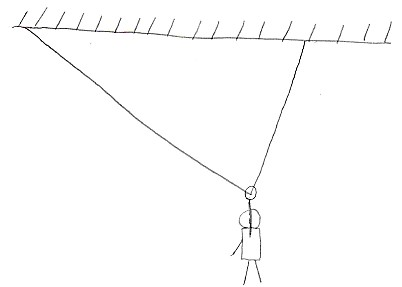
\includegraphics[height=4cm,clip]{nishimura/image/toi1.jpg}
  \caption{問1}
  \label{fig:toi1}
\end{figure}

\newpage
\section*{問2}
3月21日ころが春分の日、9月23日ころが秋分の日で\\
春分の日から秋分の日まで(春→夏→秋)は約186日\\
秋分の日から春分の日まで(秋→冬→春)は約179日\\
あります。さてこの約七日間の差はなぜ生じるのでしょうか。

\begin{description}
  \item[(A)] 歳差運動があるから冬季は一日が短いから
  \item[(B)] 冬季は一日が短いから
  \item[(C)] 太陽に近いとき、地球が速く動くから
  \item[(D)] 特に理由がない
\end{description}
※ヒント\ ケプラーの法則

\vspace{3zw}
\begin{figure}[H]
  \centering
  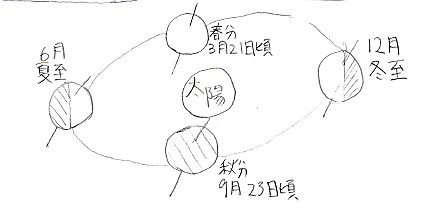
\includegraphics[height=6cm,clip]{nishimura/image/toi2.jpg}
  \caption{問2}
  \label{fig:toi2}
\end{figure}

\newpage
\section*{問3}
通常これらのうちで電磁波を放射しないのはどれでしょう。

\begin{description}
  \item[(A)] 太陽
  \item[(B)] 火山灰
  \item[(C)] 石炭
  \item[(D)] この本に使われている紙
  \item[(E)] どれも電磁波を放射している
\end{description}
※ヒント\ ウィーンの変位則
\vspace{3zw}
\begin{figure}[H]
  \centering
  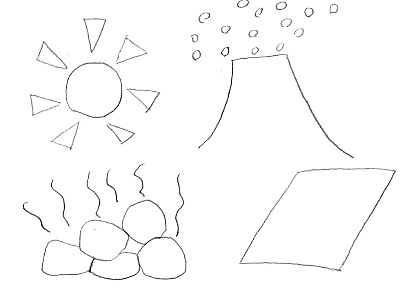
\includegraphics[height=7cm,clip]{nishimura/image/toi3.jpg}
  \caption{問3}
  \label{fig:toi3}
\end{figure}

\newpage
\section*{解答}
\section*{問1}
 解答 (B) \par
人は静かに止まっているので、人に働く外力はつりあっています。(外力は人の重力と重力の逆向きで大きさの等しい上向きの力)
ここで上向きの力はロープの左右両側の張力を合成したものです。よって下図のようになります。下図より右のロープのほうが左のロープより大きな張力が働くので右側が先に千切れます。
\begin{figure}[H]
  \centering
  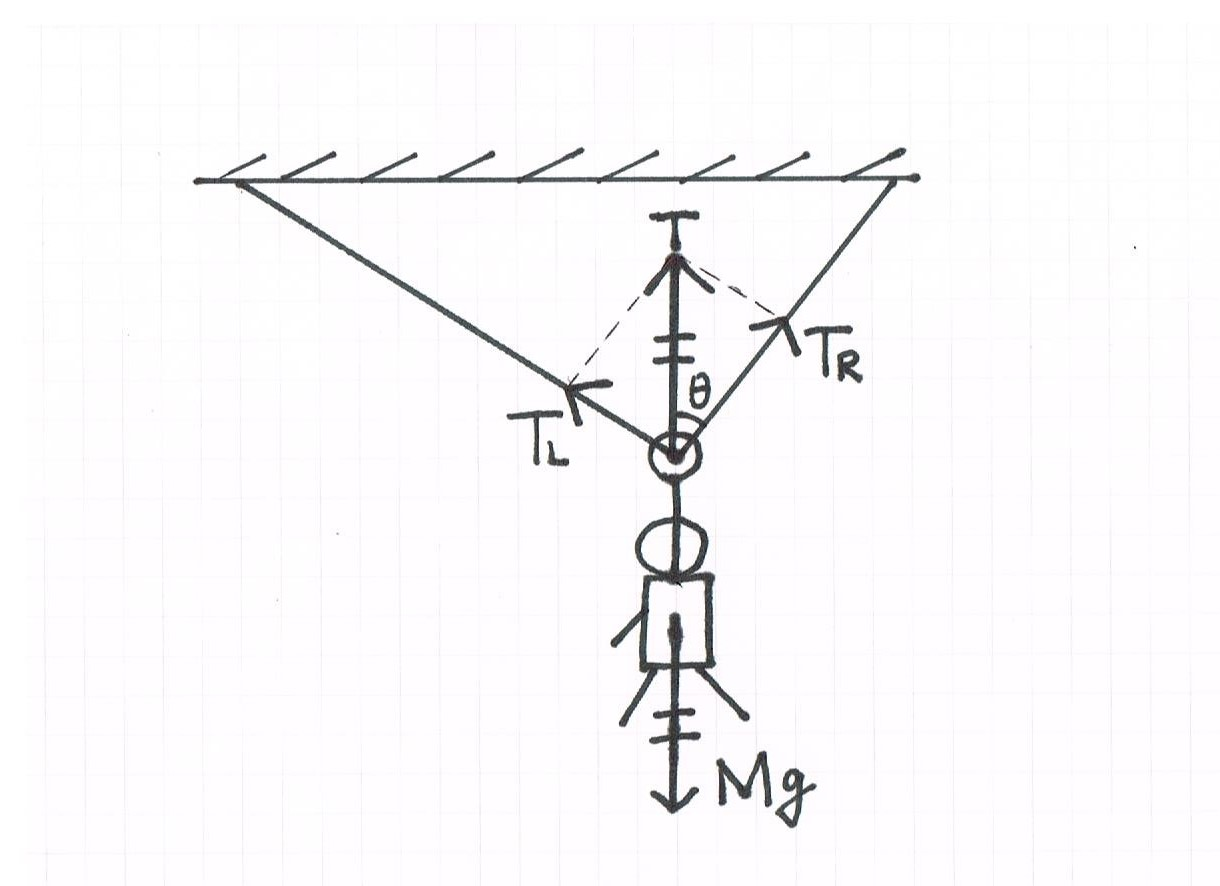
\includegraphics[height=4cm,clip]{nishimura/image/toi1_A.jpg}
  \caption{問3}
  \label{fig:toi3}
\end{figure}
この現象を数式を使って説明すると、
 人間の質量をM[kg]、重力加速度をg[$m/s^2$]とする。右側の糸に働く張力を$ T_R$[N]、左側の糸に働く張力を$T_L$[N]、二つの張力の合力をT[N]とすると、図より次の3式が得られる。
\begin{eqnarray*}
T&=&Mg\\
T_R&=&T \cos \theta\\
T_L&=&T \sin \theta\\
\end{eqnarray*}

ここで$\theta<45$度より\\
$$T \cos \theta >T \sin \theta \longrightarrow   T_R > T_L$$ \par
したがって糸が千切れるとすれば右側が切れる。

\newpage
\section*{問2}
 解答 (C) \par
ケプラーの法則
\begin{enumerate}
\item	太陽系の惑星は太陽を一つの焦点とした楕円軌道を公転する(第一法則)
\item	太陽と惑星とを結ぶ積分が単位時間に描く面積は一定である(第二法則)
\item	惑星の軌道の超半径の三乗と惑星の公転周期の二乗の比は、どの惑星に於いても一定である(第三法則)
\end{enumerate}\par
1より地球と太陽の距離は変化します。②より地球と太陽の距離が近いほど公転軌道を早く移動します。そして現在は北半球が冬の時その距離が小さくなるので冬至のころに最も移動速度が大きくなります。よって秋分→冬至→春分までの日数のほうが春分→夏至→秋分までの日数よりも短くなります。

% \newpage
\section*{問3}
 解答 (E) \par
ウィーンの変位則
物体から放射される光のうちエネルギー密度が最大になる光の波長$\lambda$は物体の本土に反比例して短くなる
\[
\lambda = \frac{k}{T}
\]
ここで$k$は比例定数、$T$は温度

すべての物質はエネルギーを電磁波として放射しています。最も多くのエネルギーを放射する電磁波の周波数を$f$とすれば、$f$と$T$には比例関係があります。この紙も例外ではなく、低温のため低周波数ではありますが、電磁波を放射しています。

\newpage
\section*{参考\ ケプラーの三法則}
\begin{description}
\item[第1法則] 惑星は太陽を一つの焦点とする楕円軌道を描く。
\item[第2法則] 惑星が太陽のまわりに描く面積速度は,各惑星毎に一定である。
\item[第3法則] 惑星の公転周期$T$の2乗は,楕円の長軸の長さaの3乗に比例する。
\end{description}
\subsection*{ケプラーの第一法則について}
ケプラーの第一法則が発見されるまでは、惑星は太陽を中心に完全な円上を運動しているとされていた。もし、軌道が完全な円だとしたら図\ref{fig:kep1}のようになる。
\begin{figure}[H]
  \centering
  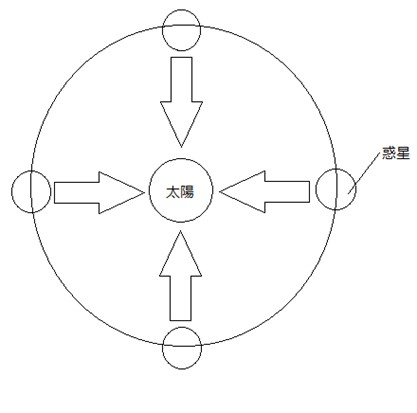
\includegraphics[height=5cm,clip]{nishimura/image/kep1.jpg}
  \caption{ケプラーの第一法則}
  \label{fig:kep1}
\end{figure}
この場合、惑星と太陽の距離はどこから測っても同じになる。
しかし、観測結果は惑星の位置によって太陽との距離が変化した。(図\ref{fig:kep1_1})\par
つまり、軌道は楕円軌道だった。
\begin{figure}[H]
  \centering
  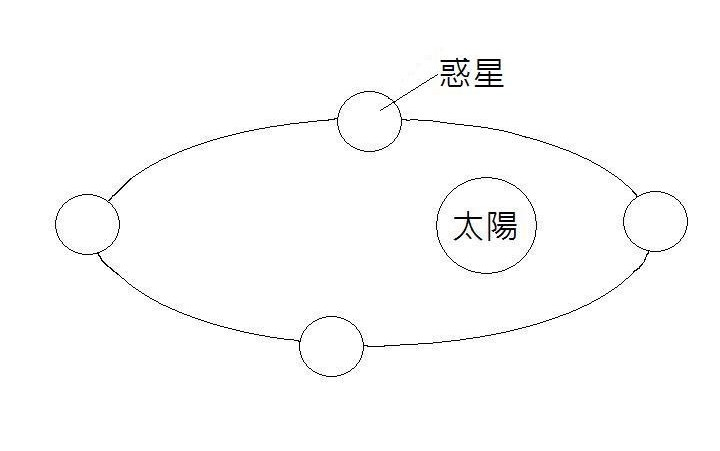
\includegraphics[height=4cm,clip]{nishimura/image/kep1_1.jpg}
  \caption{ケプラーの第一法則}
  \label{fig:kep1_1}
\end{figure}

\subsection*{ケプラーの第二法則について}
万有引力は中心に向かう力,中心力だから惑星の運動の角運動量Lは保存する。すなわち角運動量はその方向が惑星の軌道面に垂直な z 方向の成分しかなく,その大きさは極座標で表すと
\begin{eqnarray*}
L_z &=& m(xv_y-yv_x)\\
&=&mr\cos \theta \left(\frac{\rm{d}r}{\rm{d}t}\sin \theta + r\cos \theta \frac{\rm{d}\theta}{\rm{d}t}\right) - mr\sin \theta \left(\frac{\rm{d}r}{\rm{d}t}\cos \theta - r\sin \theta \frac{\rm{d}\theta}{\rm{d}t}\right) \\
&=& m r^2\frac{\rm{d}\theta}{\rm{d}t}
\end{eqnarray*}
となる。\par
したがって角運動量が一定は
\begin{eqnarray*}
L_z = m r^2\frac{\rm{d}\theta}{\rm{d}t} = D
\end{eqnarray*}
と書ける。\par
一方,面積速度は $\frac{1}{2}r^2 \frac{\rm{d}\theta}{\rm{d}t}     (=Aとする)$
であったので
\begin{eqnarray*}
\frac{1}{2}r^2 \frac{\rm{d}\theta}{\rm{d}t} = \frac{L_z}{2m} = \frac{D}{2m} = const
\end{eqnarray*}
となり,第 2 法則が導かれた。

\newpage
\subsection*{ケプラーの第三法則について}
惑星の楕円軌道の長軸 a と短軸 b はそれぞれ
\begin{eqnarray*}
\rm{a} &=&  \frac{\rm{b}^2}{a}\frac{\rm{a}^2}{\rm{b}^2} = \frac{l}{1-\epsilon ^2}\\
\rm{b} &=& \frac{\rm{b}^2}{a}\frac{\rm{a}}{\rm{b}} = \frac{l}{\sqrt{1-\epsilon ^2}}\\
\end{eqnarray*}
と表される。惑星の公転周期$T$は楕円の面積$S$を 面積速度$A$で割った時間であるから
\begin{eqnarray*}
  S = \pi \rm{ab} = \frac{\pi l^2}{(1-\epsilon ^2)^{3/2}}
\end{eqnarray*}
より
\begin{eqnarray*}
  T = \frac{S}{A} = \frac{\pi l^2}{A(1-\epsilon ^2)^{3/2}}
\end{eqnarray*}
この式の両辺を 2 乗すると
\begin{eqnarray*}
  T^2 = \frac{\pi^2 l}{A^2}\left( \frac{l}{1-\epsilon ^2}\right)^{3} = \frac{\pi^2 l \rm{a}^3}{A^2}
\end{eqnarray*}
となる。ゆえに
\begin{eqnarray*}
  \frac{T^2}{\rm{a}^3} = \frac{\pi^2}{A^2} = \frac{4\pi^2}{C}
\end{eqnarray*}
となり,ケプラーの第 3 法則が証明された。


\section*{参考文献}
\begin{enumerate}
  \item	ポール・G・ヒューイット作 松森靖夫 編著「傑作!物理パズル50」講談社 P.233
  \item	瀬戸悟「ケプラーの法則と万有引力」\\
  http://www.ishikawa-nct.ac.jp/lab/e/seto/www/files/kepler.pdf
  % HTTP://WWW.ISHIKAWA-NCT.AC.JP/LAB/E/SETO/WWW/FILES/KEPLER.PDF
\end{enumerate}
 \clearpage

\chapter*{}
\vspace{10zw} % 高さ調整
\begin{center}
  \textgt{
    {\Huge 第II部} \\ \vspace{15pt}
    {\Huge 君の長さは。} \\ \vspace{20pt}
    {\Large 理工学部 物理科学科} \\ \vspace{5pt}
    {\Large 中山敦貴} \vspace{40pt}
  }
\end{center}
\addcontentsline{toc}{part}{第II部 君の長さは。 \\ \hspace{4zw}{\small 理工学部 物理科学科 中山 敦貴}}
\newpage
\section*{はじめに}
バネで定在波を作って遊んでいるとき、振幅が最大のときのバネは振幅0のときに比べてどれぐらい伸びているのか気になったので調べてみた。波形はサインカーブであるから、サインの曲線に沿った長さを求めればよい。\par
ついでにカテナリー曲線についても調べた。これも日常よく見る曲線であり、知っておいて損はないかと思われる。

\chapter{サインカーブ}

\section{サインカーブの長さ}
\vspace{1zw}
\begin{center}
  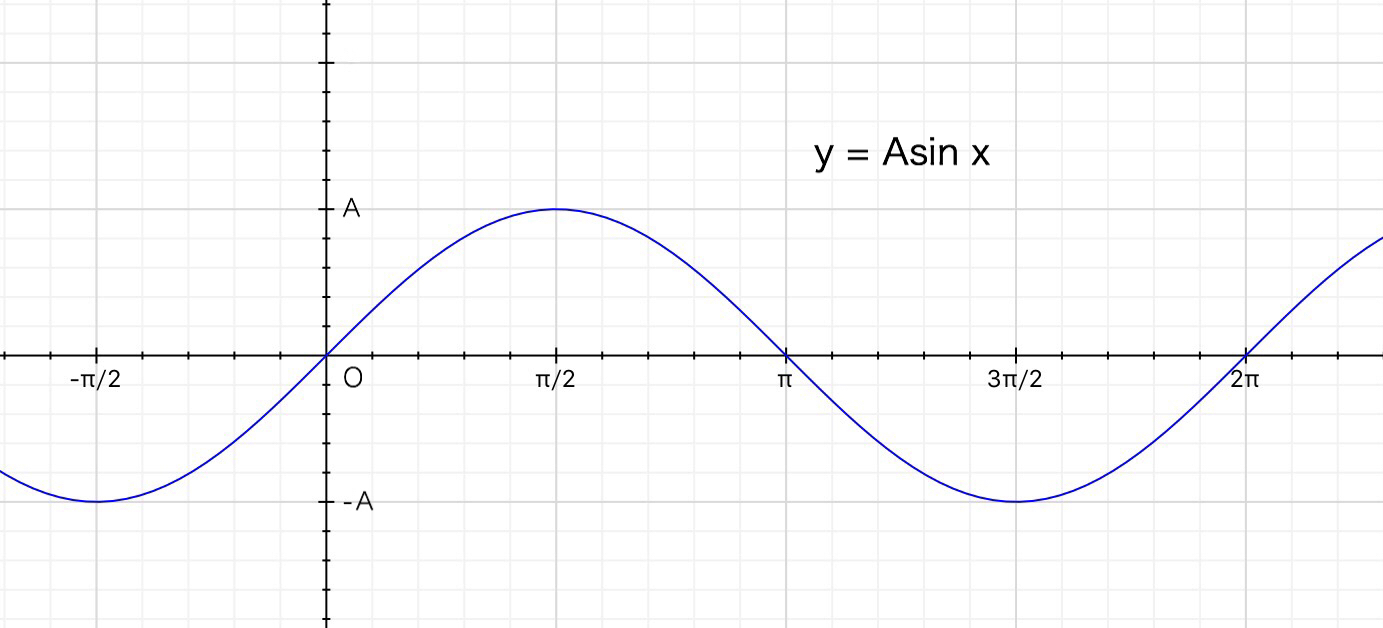
\includegraphics[width = 12cm]{nakayama/image/sine3.JPG}
\end{center}
\vspace{1zw}\par
$y = A \sin x$の曲線の長さを求めよう。求める長さを$L$とする。\par
\begin{wrapfigure}{r}{40mm}
\begin{center}
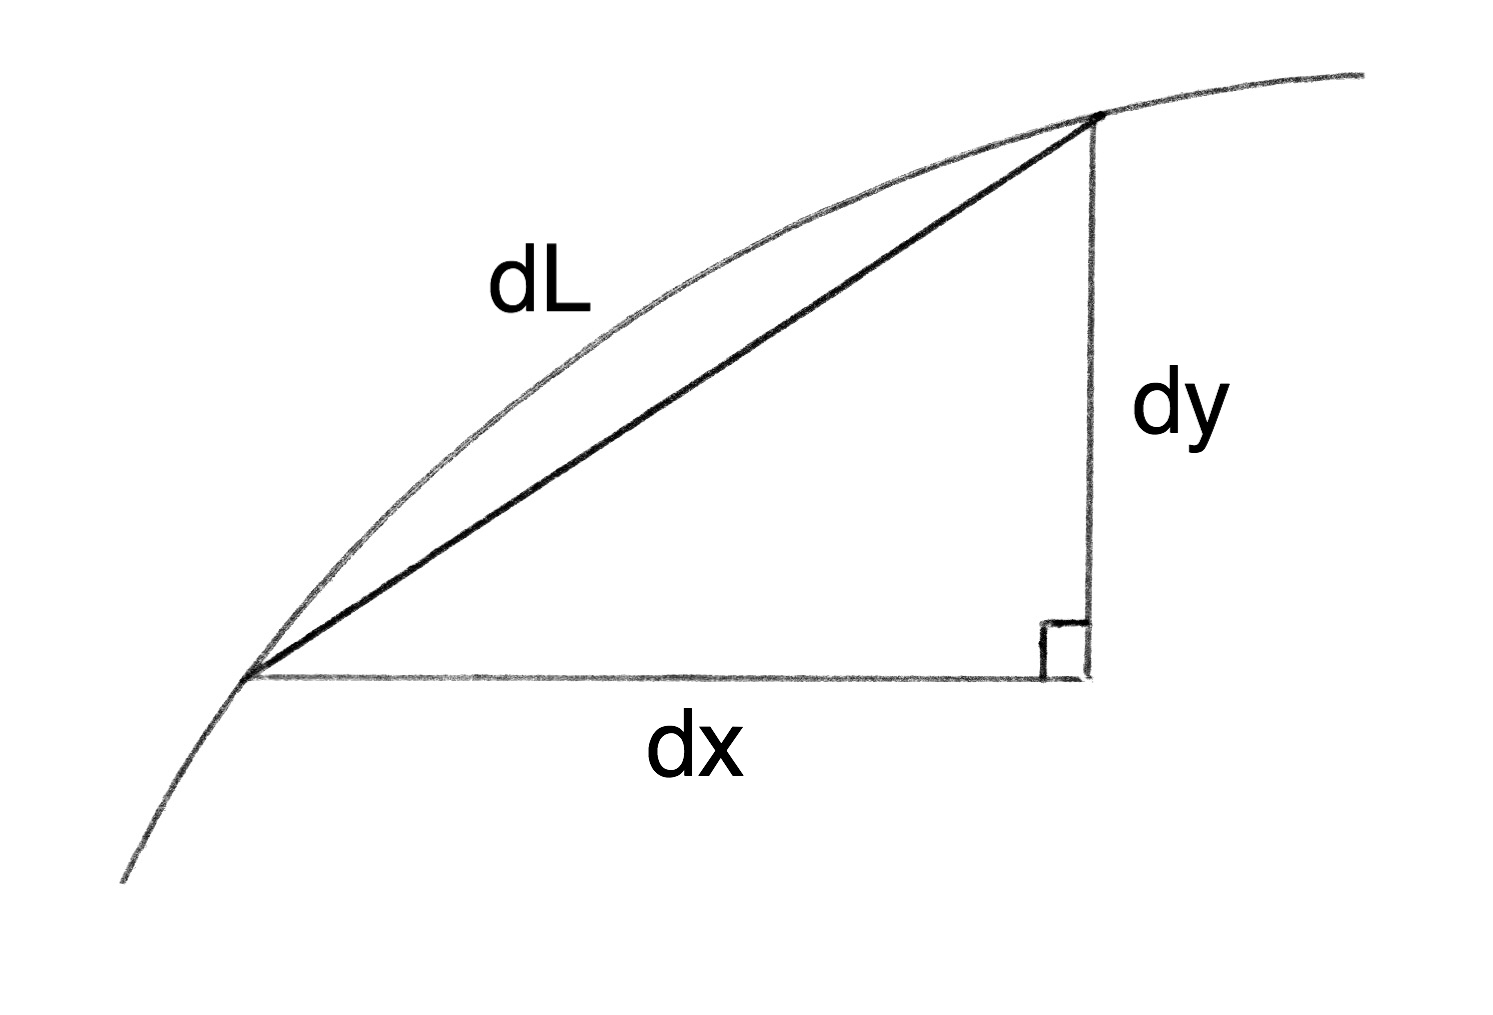
\includegraphics[width = 4cm]{nakayama/image/dL.jpg}
\end{center}
\end{wrapfigure}
微小長さ$dL$は三平方の定理より

\begin{eqnarray*}
dL & = & \sqrt{(dx)^2 + (dy)^2} \\
& = & \sqrt{1 + \left(\frac{dy}{dx}\right)^2}\,\,dx.
\end{eqnarray*}
\newline\par
よって
\begin{eqnarray*}
L & = & \int_{x_1}^{x_2} \sqrt{1 + \left(\frac{dy}{dx}\right)^2}\,\,dx \\
& = & \int_{x_1}^{x_2} \sqrt{1 + (A\cos x)^2}\,\,dx.
\end{eqnarray*}

あとはこれを計算するだけだが、どうにもこの積分は計算できそうにない。\par
もう少し変形してみると
\begin{eqnarray*}
L & = & \int_{x_1}^{x_2} \sqrt{1 + A^2(1 - \sin^2 x)}\,\,dx \\
& = & \int_{x_1}^{x_2} \sqrt{1 + A^2 - A^2\sin^2 x}\,\,dx \\
& = & \sqrt{A^2 + 1} \int_{x_1}^{x_2} \sqrt{1 - \frac{A^2}{A^2 + 1}\sin^2 x}\,\,dx
\end{eqnarray*}
となるが、この積分は第二種の楕円積分と呼ばれるもので、初等的には計算できないらしい。しかし、積分区間を$x =0〜\frac{\pi}{2}$とすることでなんとか級数の形にまでもっていくことができる。まずは次の2つの公式を用意しよう。


\section{準備}

\subsection{二項展開}

次の左辺は$|X| < 1$の条件のもとで
\begin{eqnarray*}
(1 - X)^a = \sum_{k=0}^\infty (-1)^k \binom{a}{k} X^k
\end{eqnarray*}
とテイラー展開できる\footnote{$a > 0$の場合、$X = \pm1$のときも収束する。}。\par
ここで$\binom ak$はコンビネーション$_aC_k$の$a$を実数の範囲にまで拡張したものであり
\begin{eqnarray*}
\binom ak = \frac{a(a-1)(a-2)\cdots(a-(k - 1))}{k!}
\end{eqnarray*}
と定義されている。ただし
$$
\binom a0 = 1
$$
とする。\par
上の式で$a = \frac{1}{2}$とすると
\begin{eqnarray*}
(1 - X)^\frac{1}{2} & = & \sum_{k=0}^\infty (-1)^k \binom{\frac{1}{2}}{k} X^k \\
& = & \binom{\frac{1}{2}}{0} + \sum_{k=1}^\infty (-1)^k \frac{\frac{1}{2} \left(\frac{1}{2} - 1 \right)\left(\frac{1}{2}-2\right) \cdots \left(\frac{1}{2} - (k - 1)\right)}{k!} X^k \\
& = & 1 + \sum_{k=1}^\infty (-1)^k \frac{\frac{1}{2} \left(-\frac{1}{2} \right)\left(-\frac{3}{2}\right) \cdots \left(-\frac{2k - 3}{2}\right)}{k!} X^k \\
& = & 1 + \sum_{k=1}^\infty (-1)^k\frac{(-1)^{k - 1}(2k - 3)\cdots3\cdot1}{2^k \cdot k!} X^k \\
& = & 1 - \sum_{k=1}^\infty \frac{(2k - 3)!!}{(2k)!!}  X^k
\end{eqnarray*}
を得る。ただし$(-1)!! = 1$と定義する。

\subsection{$\sin^Nx$の積分}

部分積分と漸化式を用いて$I_N = \int_0^{\frac{\pi}{2}}\sin^N x\,dx$を計算する。
\begin{eqnarray*}
I_N & = & \int_0^{\frac{\pi}{2}}\sin^N x\,dx \\
& = & \int_0^{\frac{\pi}{2}}\sin x \, \sin^{N - 1}x \,dx \\
& = & \int_0^{\frac{\pi}{2}}(-\cos x)^{'} \sin^{N - 1}x \,dx \\
& = & [-\cos x\,\sin^{N - 1}x]_0^\frac{\pi}{2} - \int_0^{\frac{\pi}{2}}(-\cos x)(N -1)\sin^{N - 2}x \cos x\,dx \\
& = & 0 + (N - 1)\int_0^{\frac{\pi}{2}}\cos^2 x\,\sin^{N - 2}x\,dx \\
& = & (N - 1)\int_0^{\frac{\pi}{2}}(1 - \sin^2x)\,\sin^{N - 2}x\,dx \\
& = & (N - 1)\int_0^{\frac{\pi}{2}}(\sin^{N - 2}x - \sin^Nx)\,dx \\
& = & (N - 1)\,I_{N - 2} - (N - 1)\,I_N.
\end{eqnarray*}

よって、以下の漸化式が成立する。
\begin{eqnarray*}
I_N = \frac{N - 1}{N}\,I_{N - 2}.
\end{eqnarray*}

$I_0=\frac{\pi}{2}$であるから、Nが偶数のとき
\begin{eqnarray*}
I_N & = & \frac{N - 1}{N}\,I_{N - 2} \\
& = & \frac{N - 1}{N}\frac{N - 3}{N - 2}\,I_{N - 4} \\
& = & \cdots \quad=\,\,\, \frac{(N - 1)!!}{N!!}\,I_0 \\
& = & \frac{(N - 1)!!}{N!!}\frac{\pi}{2}
\end{eqnarray*}
となる。


\section{サインカーブの長さ 続き}

\subsection{楽しい計算}

準備が整った。これでようやく積分の続きが計算できる。ただし積分区間は$x=0〜\frac{\pi}{2}$とする。
\begin{eqnarray*}
L & = & \sqrt{A^2 + 1} \int_0^\frac{\pi}{2} \sqrt{1 - \frac{A^2}{A^2 + 1}\sin^2 x}\,\,dx \\
& = & \sqrt{A^2 + 1} \int_0^\frac{\pi}{2} \left(1 - \frac{A^2}{A^2 + 1}\sin^2 x \right)^\frac{1}{2}\,dx
\end{eqnarray*}
$|\frac{A^2}{A^2 + 1}\sin^2 x| \leq 1$であるから、2.2.1より
\begin{eqnarray*}
\qquad\qquad\qquad\quad & = & \sqrt{A^2 + 1} \int_0^\frac{\pi}{2}\left(1 - \sum^{\infty}_{k = 1}\frac{(2k - 3)!!}{(2k)!!}\left(\frac{A^2}{A^2 + 1}\sin^2 x\right)^k\,\right)dx \\
& = & \sqrt{A^2 + 1} \left(\int_0^\frac{\pi}{2}dx - \sum^{\infty}_{k = 1}\frac{(2k - 3)!!}{(2k)!!}\left(\frac{A^2}{A^2 + 1}\right)^k \int_0^\frac{\pi}{2}\sin^{2k}x\,dx \right)
\end{eqnarray*}
2.2.2より
\begin{eqnarray*}
\qquad\qquad\qquad\quad & = & \sqrt{A^2 + 1} \left(\frac{\pi}{2} - \sum^{\infty}_{k = 1}\frac{(2k - 3)!!}{(2k)!!}\left(\frac{A^2}{A^2 + 1}\right)^k\frac{(2k - 1)!!}{(2k)!!}\frac{\pi}{2} \right)\\
& = & \frac{\pi}{2}\sqrt{A^2 + 1} \left(1 - \sum^{\infty}_{k = 1}\frac{(2k - 1)!!}{(2k)!!(2k - 1)}\left(\frac{A^2}{A^2 + 1}\right)^k\frac{(2k - 1)!!}{(2k)!!}\right) \\
& = & \frac{\pi}{2}\sqrt{A^2 + 1} \left(1 + \sum^{\infty}_{k = 1}\left(\frac{(2k - 1)!!}{(2k)!!}\right)^2 \left(\frac{A^2}{A^2 + 1}\right)^k\frac{1}{1 - 2k} \right) \\
& = & \frac{\pi}{2}\sqrt{A^2 + 1}\,\sum^{\infty}_{k = 0}\left(\frac{(2k - 1)!!}{(2k)!!}\right)^2 \left(\frac{A^2}{A^2 + 1}\right)^k\frac{1}{1 - 2k}.
\end{eqnarray*}

これで$L$を級数で表すことができた。

\subsection{具体的な数値}

$\displaystyle L = \frac{\pi}{2}\sqrt{A^2 + 1}\,\sum^{n}_{k = 0}\left(\frac{(2k - 1)!!}{(2k)!!}\right)^2\left(\frac{A^2}{A^2 + 1}\right)^k\frac{1}{1 - 2k}$で近似を計算した。表の値は小数点以下7桁目を四捨五入している。参考までに、$\frac{\pi}{2}=1.570596...$ である。\\

\begin{table}[ht]
\begin{center}
\begin{tabular}{cc}

\begin{minipage}{0.5\hsize}
\begin{center}
A = 1 \\
\begin{tabular}{c|c} \hline
n & L \\ \hline
1 & 1.943761 \\
2 & 1.917729 \\
3 & 1.912305 \\
4 & 1.910822 \\
5 & 1.910355 \\
6 & 1.910195 \\
7 & 1.910136 \\
8 & 1.910114 \\
9 & 1.910105 \\
10 & 1.910101 \\ \hline
正確な値 & 1.9100988945... \\ \hline
\end{tabular}
\end{center}
\end{minipage}

\begin{minipage}{0.5\hsize}
\begin{center}
A = 2 \\
\begin{tabular}{c|c} \hline
n & L \\ \hline
1 & 2.809926 \\
2 & 2.704554 \\
3 & 2.669430 \\
4 & 2.654063 \\
5 & 2.646318 \\
6 & 2.642058 \\
7 & 2.639572 \\
8 & 2.638057 \\
9 & 2.637103 \\
10 & 2.636487 \\ \hline
正確な値 & 2.6351835815... \\ \hline
\end{tabular}
\end{center}
\end{minipage}

\end{tabular}
\end{center}
\end{table}

\begin{table}[htb]
\begin{center}
\begin{tabular}{cc}

\begin{minipage}{0.5\hsize}
\begin{center}
A = 0.3 \\
\begin{tabular}{c|c} \hline
n & L \\ \hline
1 & 1.606107 \\
2 & 1.605583 \\
3 & 1.605565 \\
4 & 1.605564 \\
5 & 1.605564 \\ \hline
正確な値 & 1.6055641558... \\ \hline
\end{tabular}
\end{center}
\end{minipage}

\begin{minipage}{0.5\hsize}
\begin{center}
A = 0.5 \\
\begin{tabular}{c|c} \hline
n & L \\ \hline
1 & 1.668393 \\
2 & 1.665101 \\
3 & 1.664826 \\
4 & 1.664796 \\
5 & 1.664792 \\ \hline
正確な値 & 1.664791805... \\ \hline

\end{tabular}
\end{center}
\end{minipage}

\end{tabular}
\end{center}
\end{table}

\clearpage
\section{(参考)楕円積分}
$$
E(x, m) = \int_0^x \sqrt{1 - m\sin^2 \theta}\,\,d\theta
$$
を第二種楕円積分という。また、$x = \frac{\pi}{2}$としたものを第二種完全楕円積分という。
$$
E(m) = E\left(\frac{\pi}{2}, m\right) = \int_0^\frac{\pi}{2} \sqrt{1 - m\sin^2 \theta}\,\,d\theta.
$$ \par
これを使うと、先ほど求めた$y = A\sin x$の曲線の長さ$L$は
$$
L = \sqrt{1 + A^2}\,\,E\left(\frac{A^2}{1 + A^2}\right)
$$
と書くことができる。\par
楕円積分には他にも第一種、第三種がある。振り子の周期を計算するときには第一種の楕円積分が出てくる。暇な人は計算してみるとよい。

\chapter{カテナリー曲線}
\section{カテナリー曲線とは}
ロープや電線などの両端を持って垂らしたときにできる曲線のことをカテナリー曲線または懸垂曲線という。\\
\begin{center}
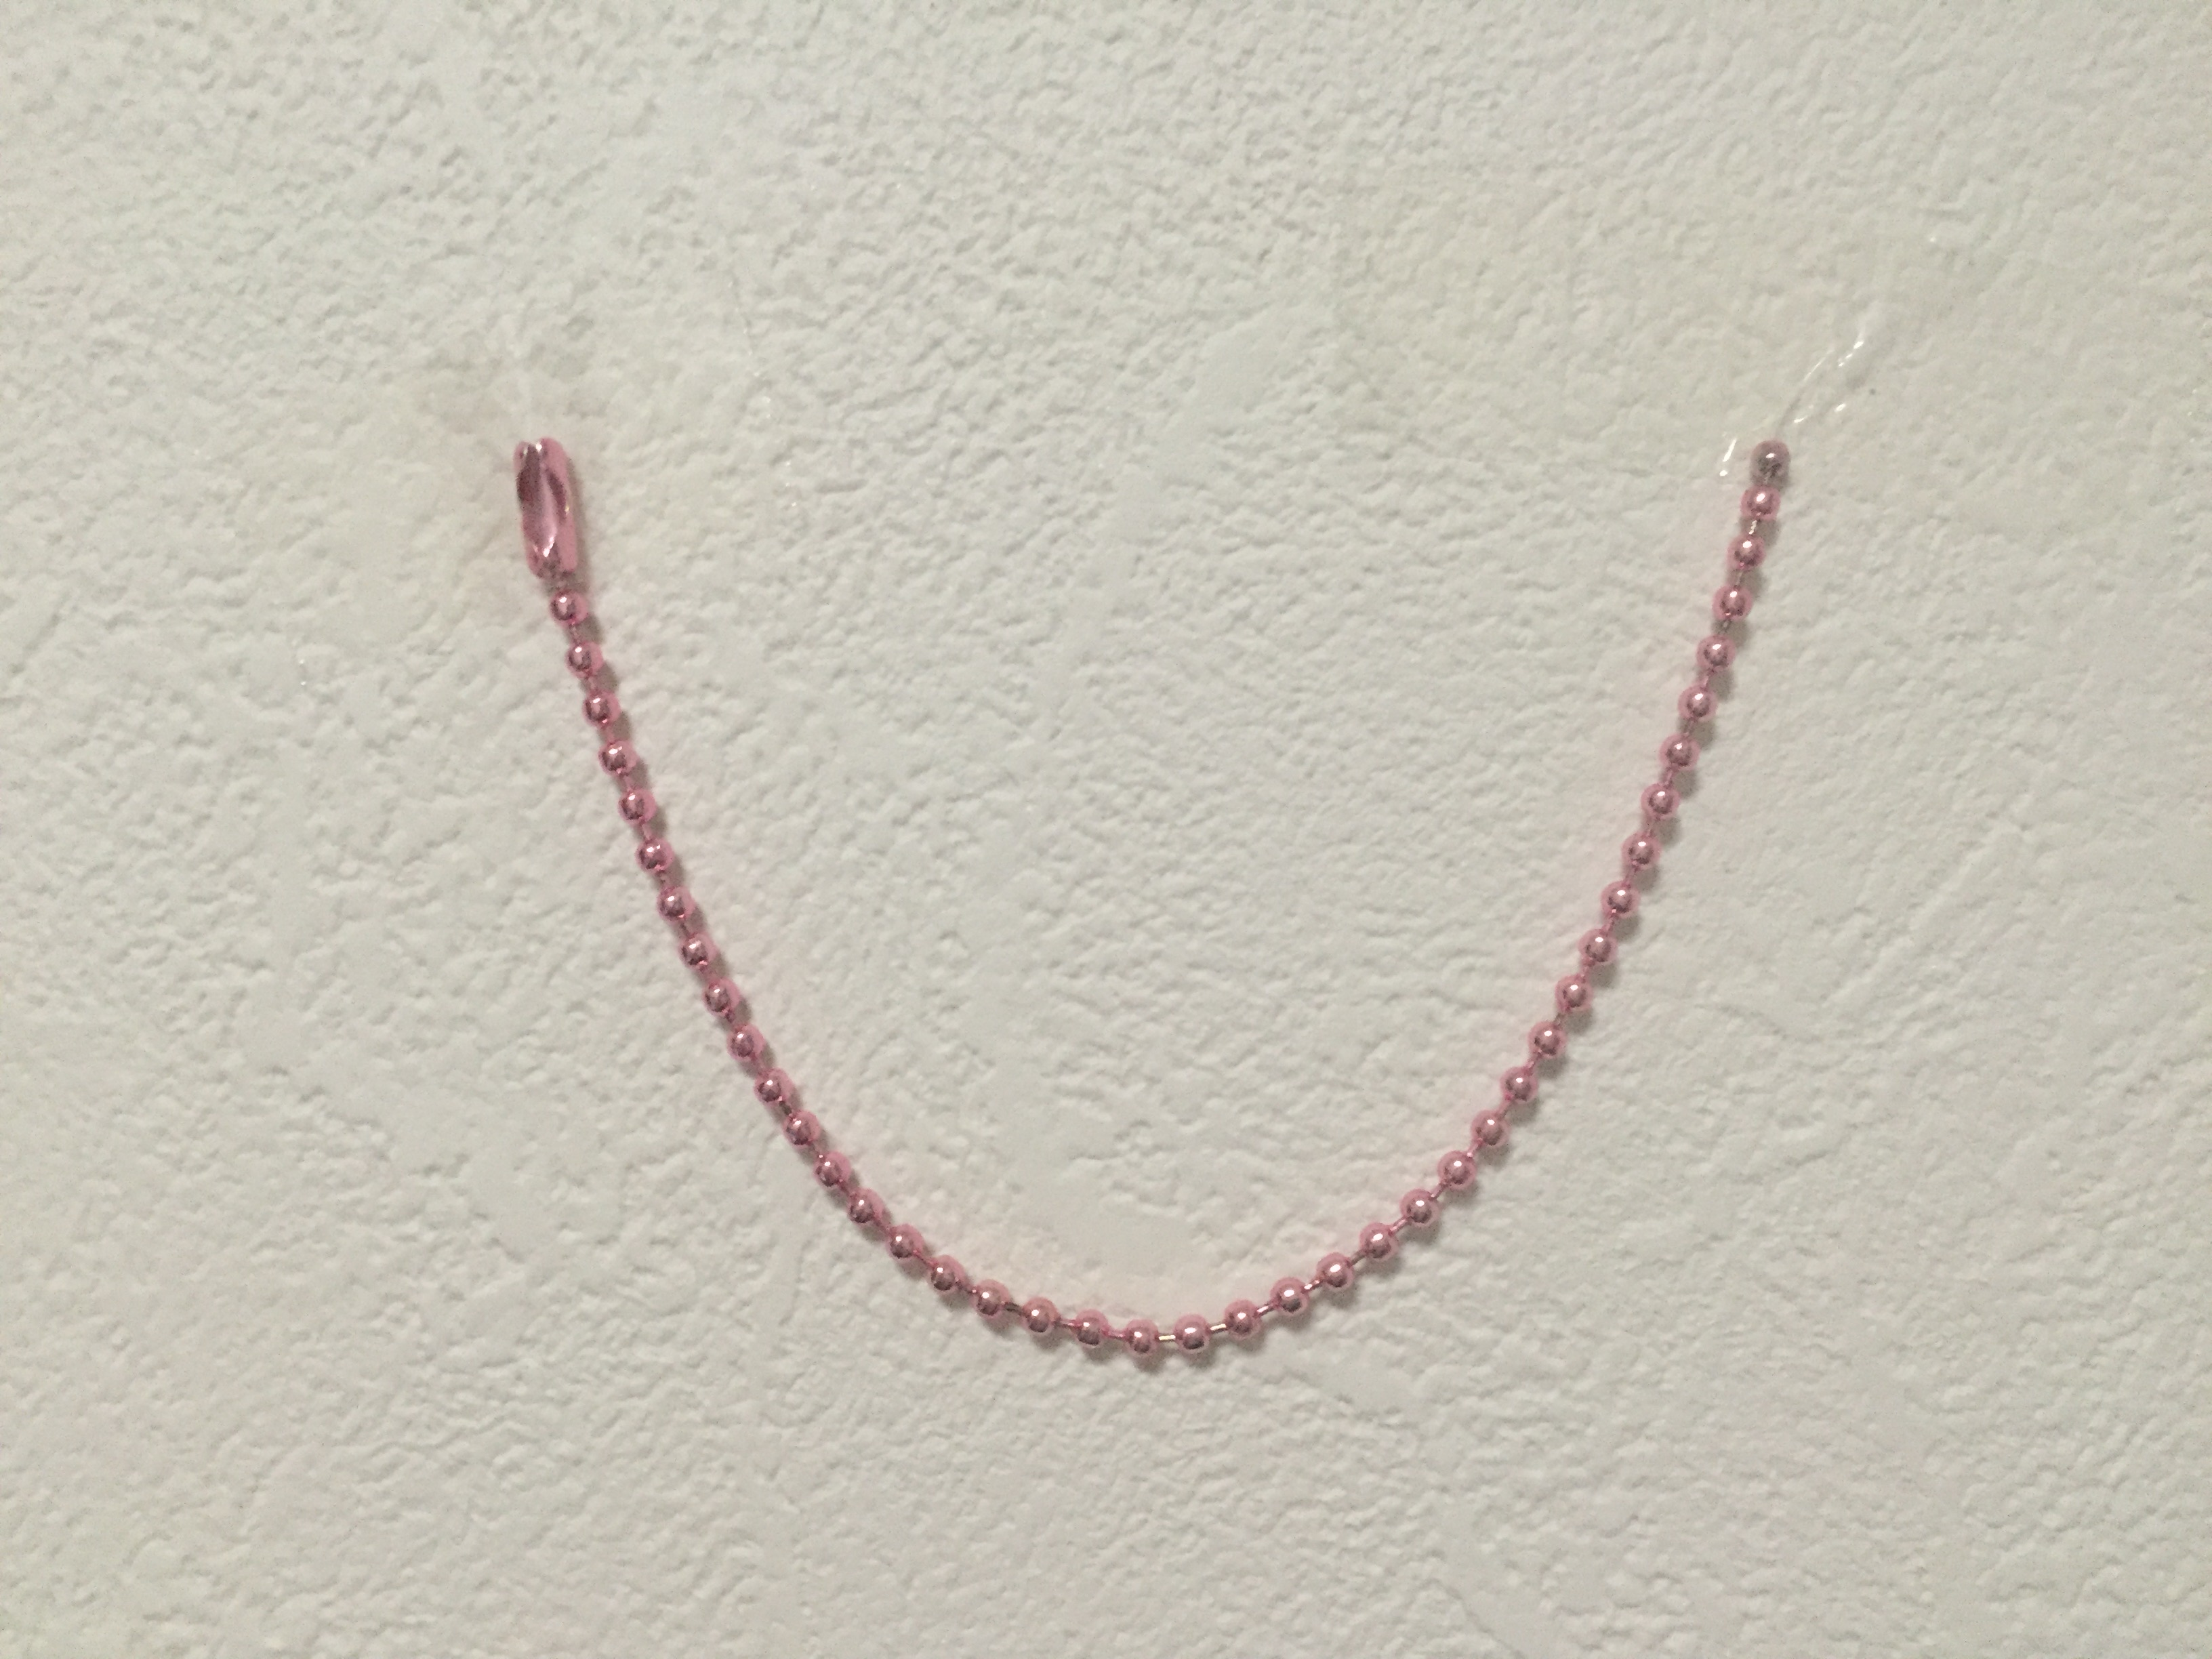
\includegraphics[width = 5cm]{nakayama/image/chen.JPG}
\quad
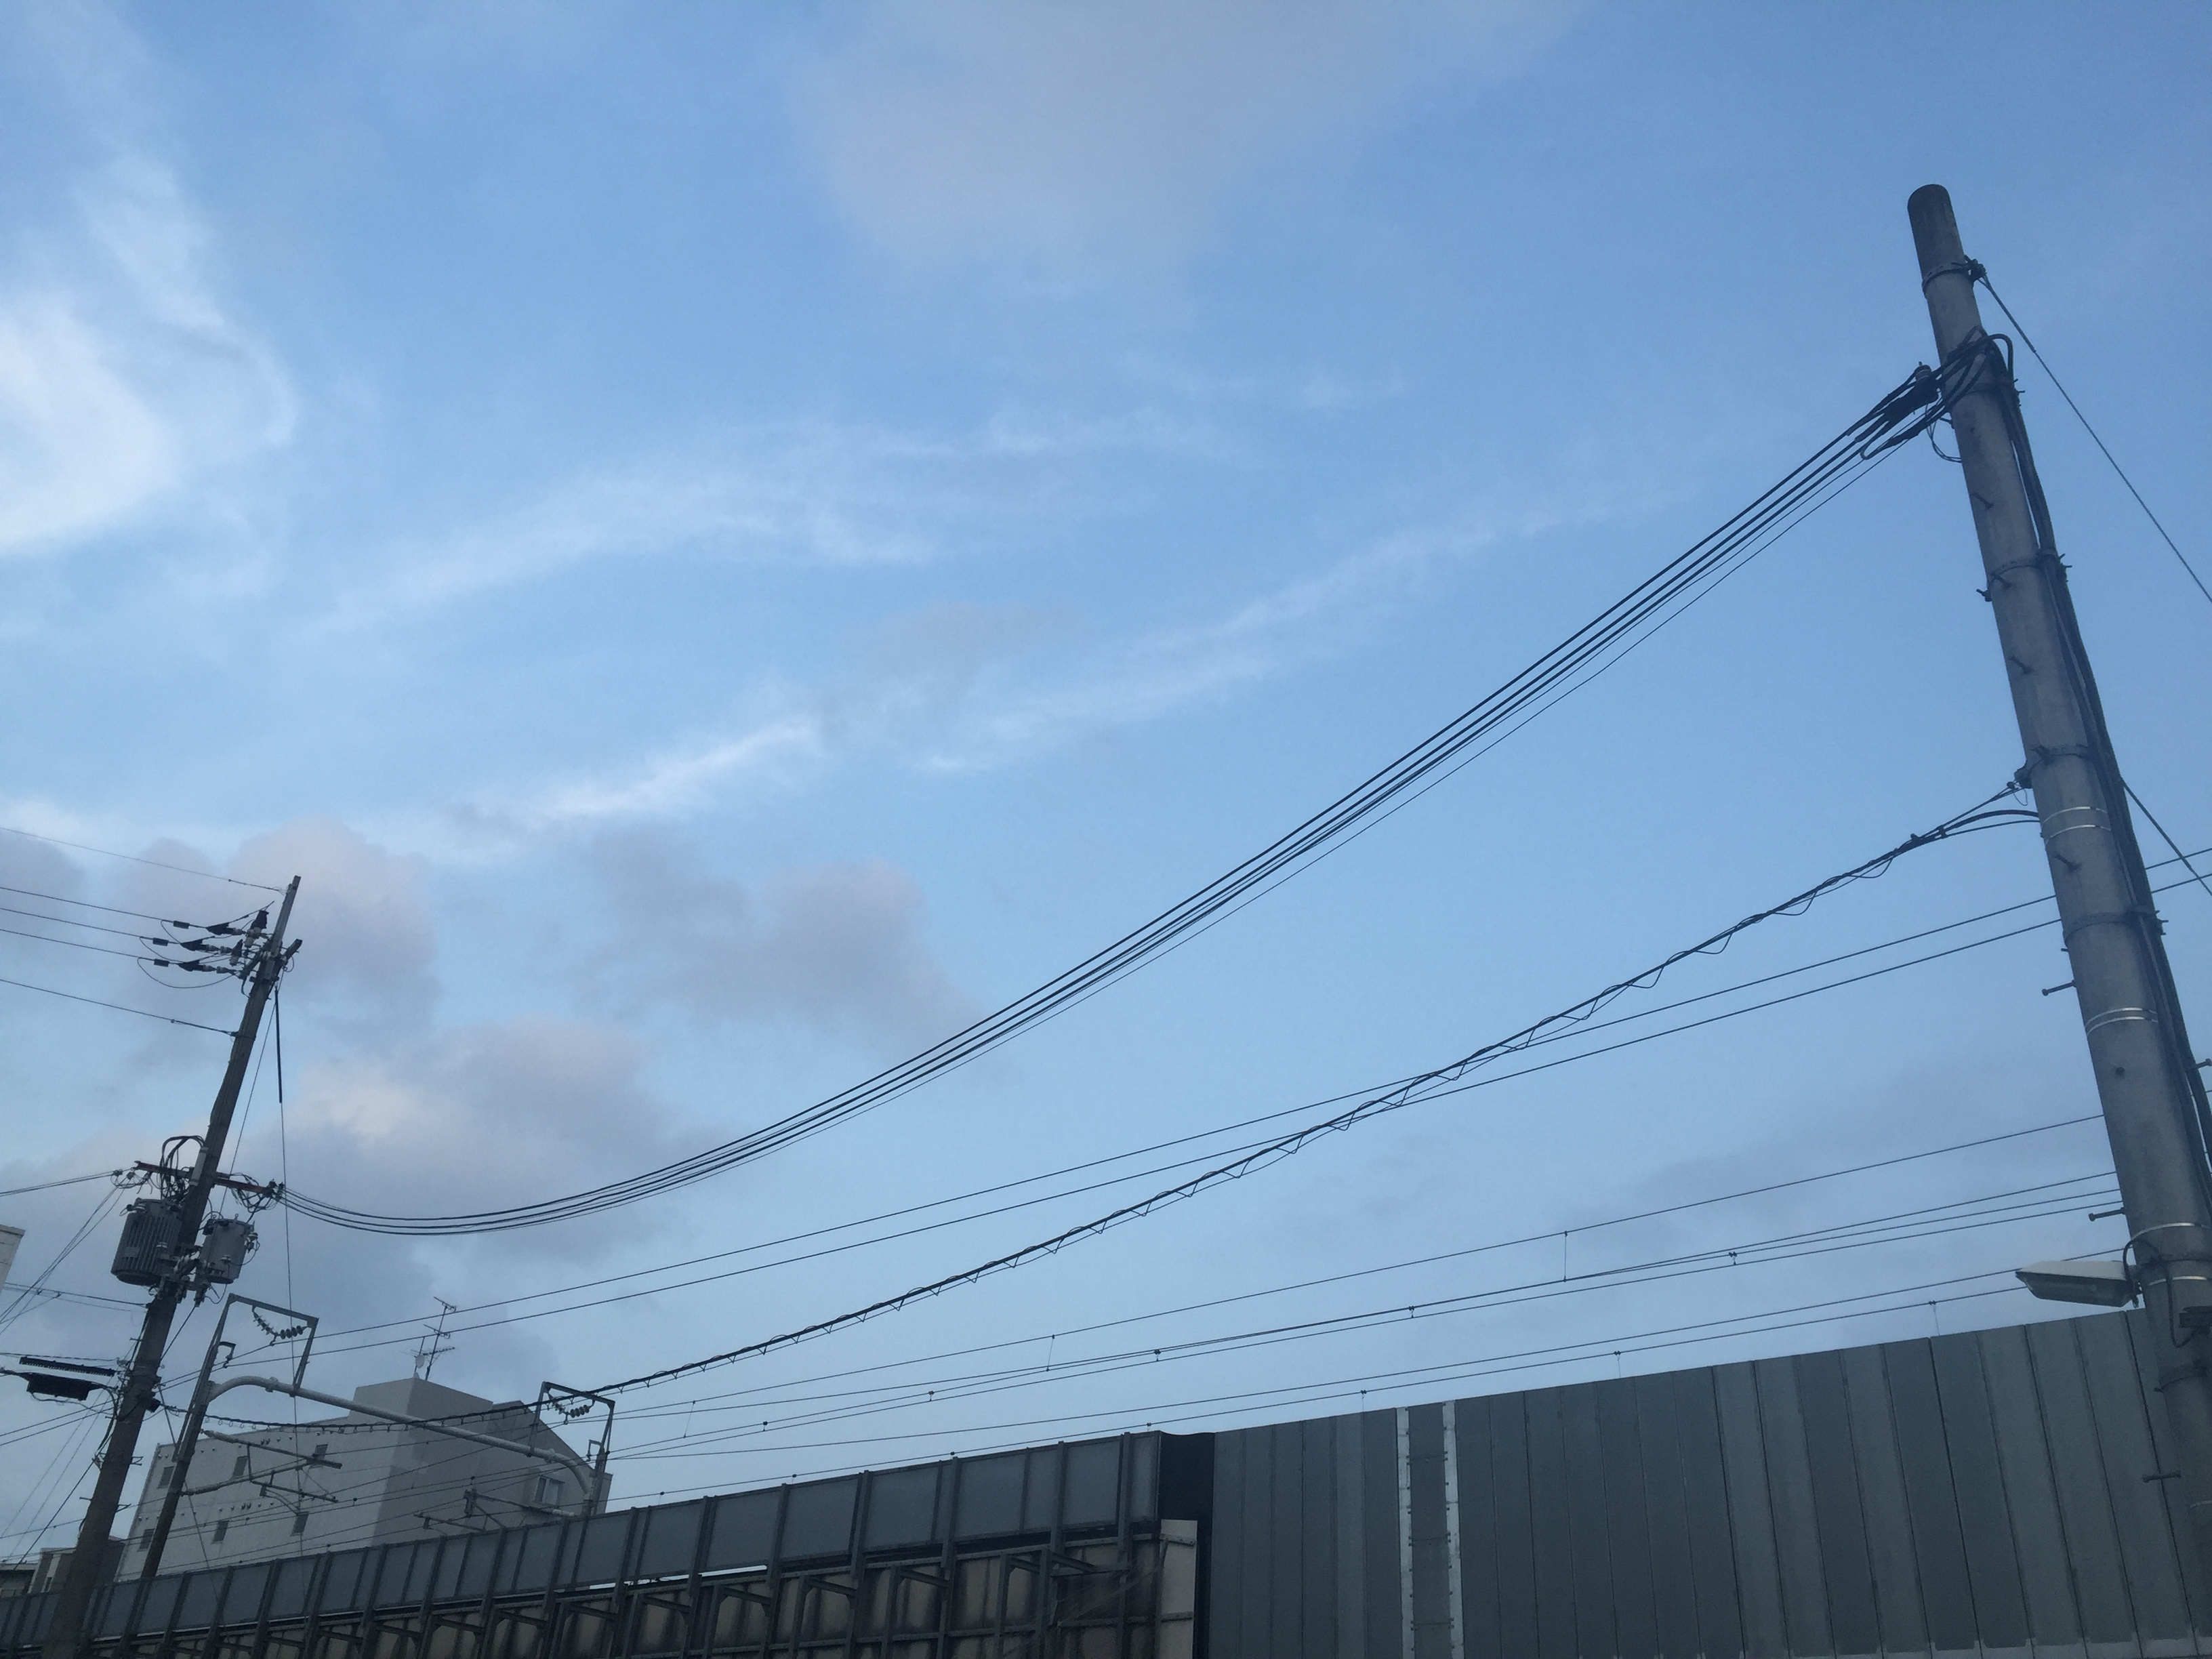
\includegraphics[width = 5cm]{nakayama/image/densen.JPG}
\end{center}

\section{曲線の方程式}
まずはカテナリー曲線の方程式を求める。曲線は、頂点における法線を軸として線対称であり、一様な質量の線密度を持つものと仮定する。

カテナリー上で頂点($x$座標を$0$とする)からの弧長が$s$であるような点$(x, y)$において、その接線が$x$軸の正の向きと成す角を$\theta$と置くとき、頂点から点$(x, y)$までの弧に掛かる力の釣り合いを考える。重力加速度を$g$、曲線の線密度を$w$とすれば、点$(x, y)$における張力$T$の鉛直成分 $T\sin{\theta}$は、頂点から点$(x, y)$までの弧にかかる重力$wgs$と釣り合う。また、頂点における張力は水平成分のみであり、この大きさを$k$とすると、点$(x,y)$における張力の水平成分$T\cos{\theta}$と釣り合う。
\begin{center}
  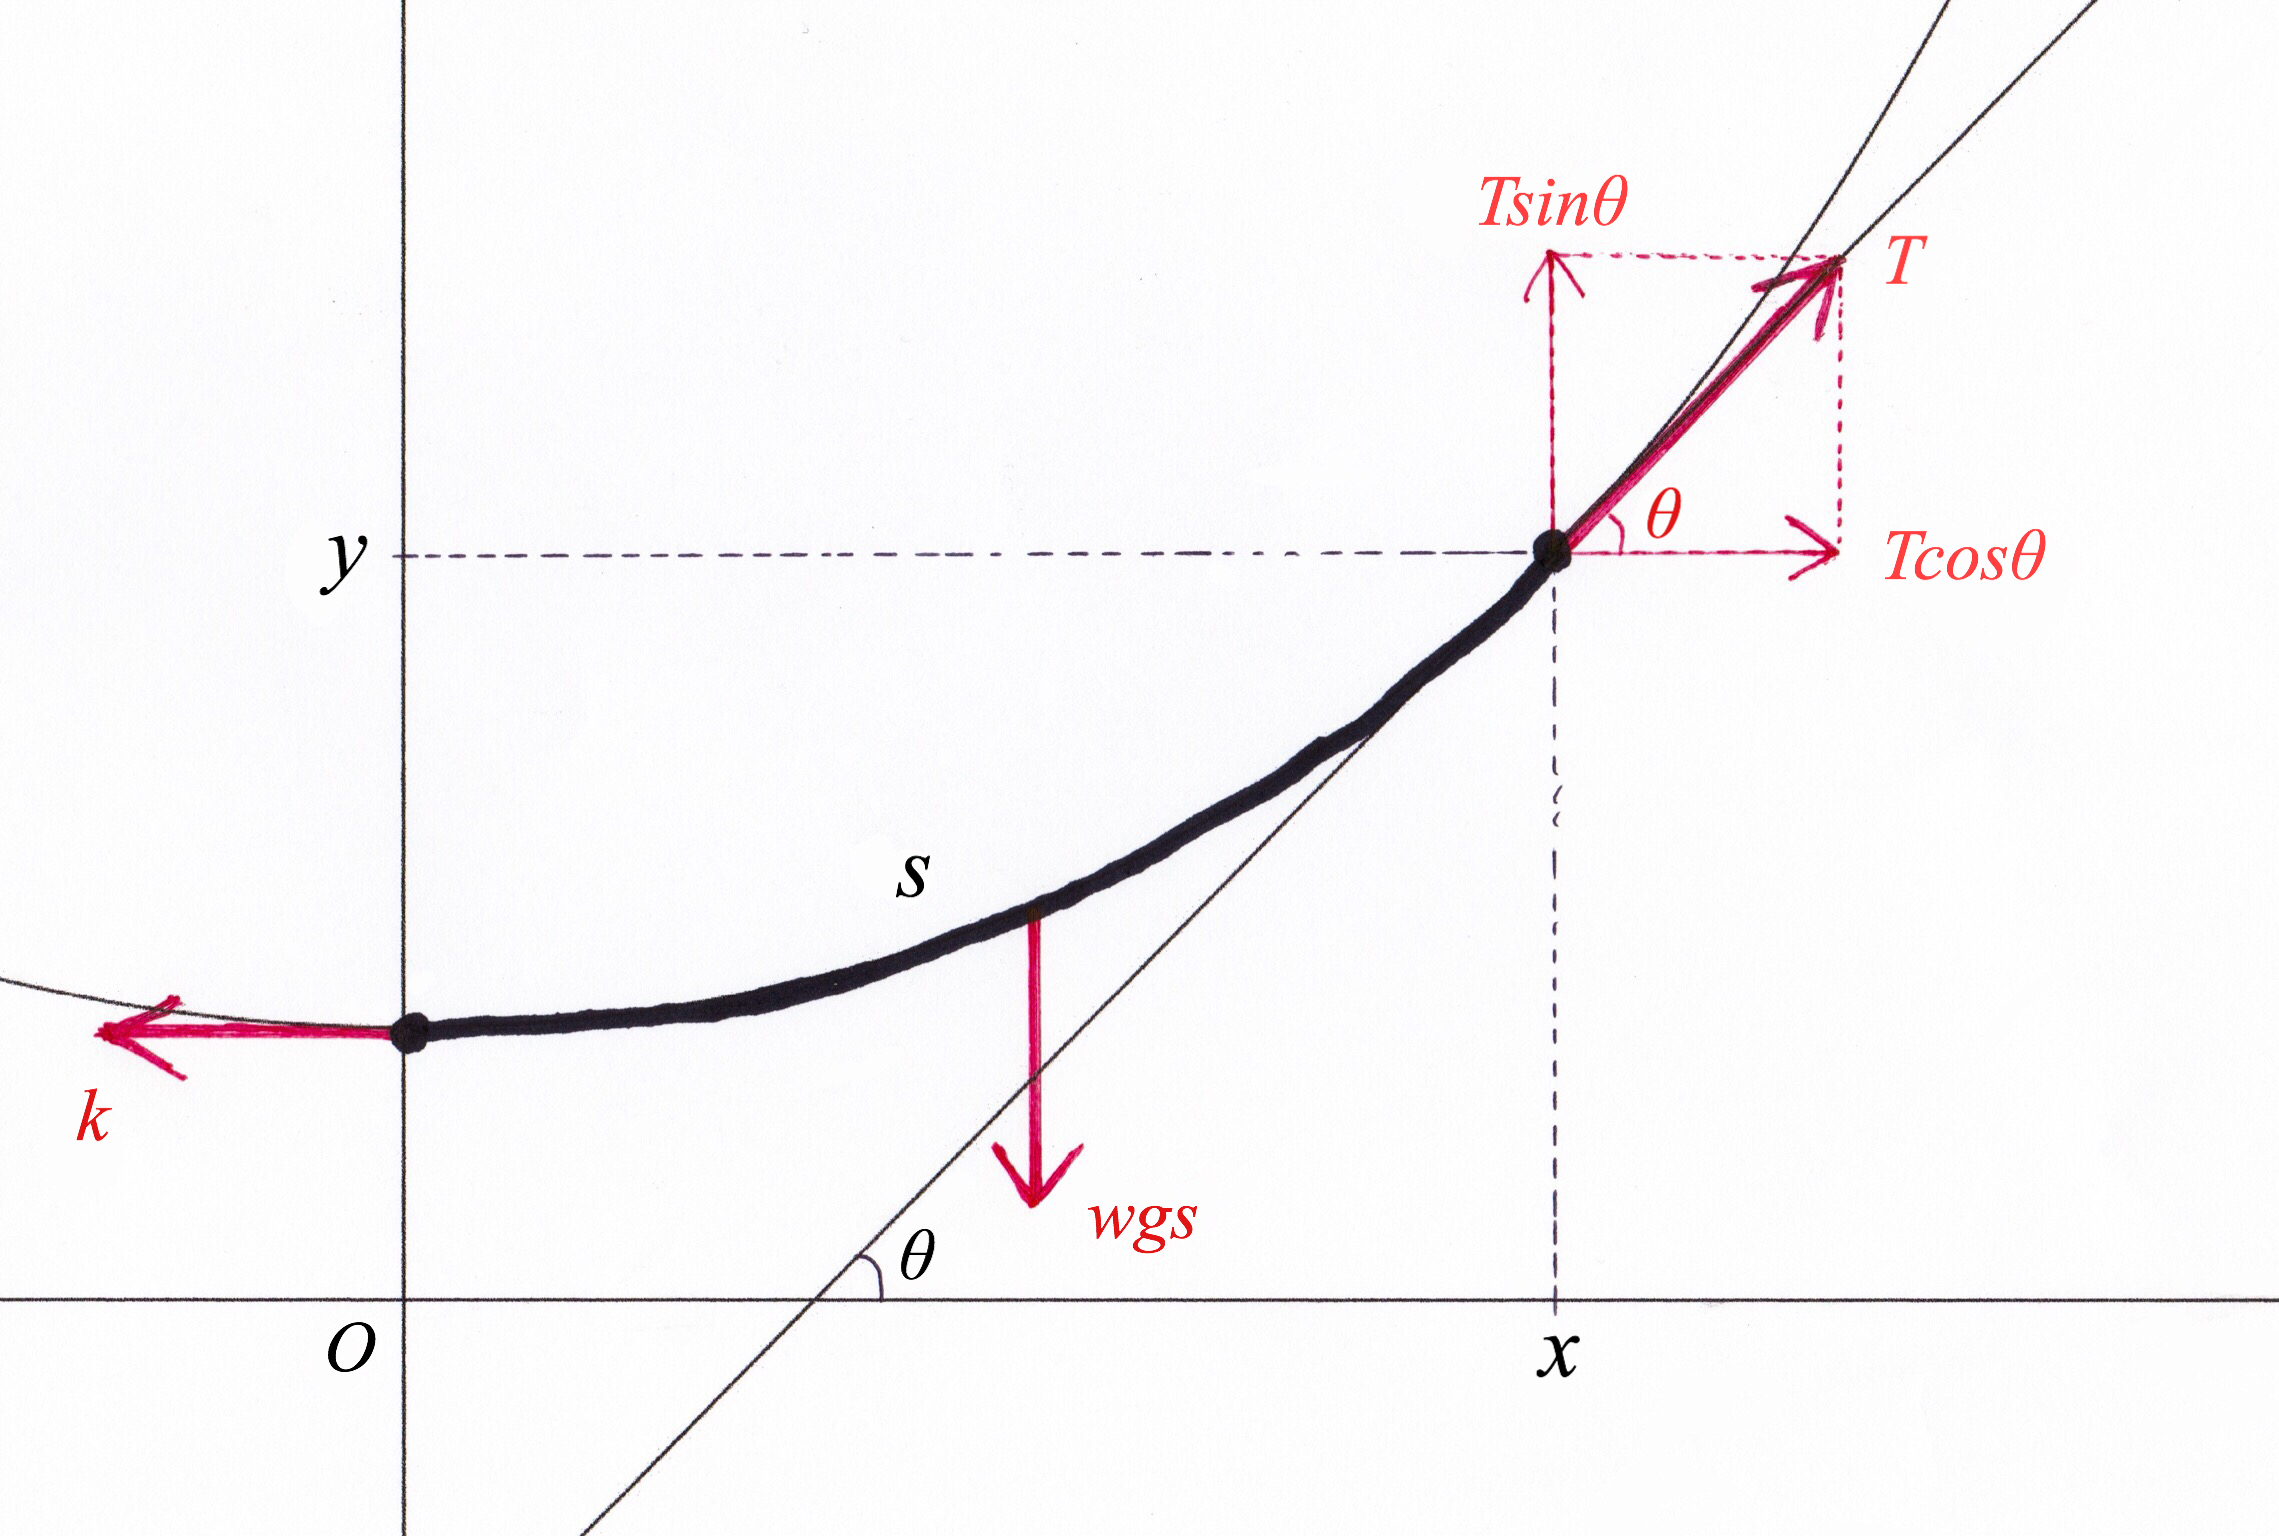
\includegraphics[width = 8cm]{nakayama/image/catenary2.JPG}
\end{center}
\vspace{-0.5zw}
\begin{displaymath}
\left\{
\begin{array}{l}
T\sin{\theta} = wgs \\
T\cos{\theta} = k \\
\tan{\theta} = \dfrac{dy}{dx}
\end{array}
\right.
\end{displaymath}
という条件が得られるので、これを解く。\\

3式から
\begin{eqnarray*}
\tan{\theta} = \frac{dy}{dx} = \frac{wgs}{k}.
\end{eqnarray*}

$\frac{k}{wg} = a$とおいて
\begin{eqnarray*}
\frac{dy}{dx} & = & \frac{s}{a}.
\end{eqnarray*}

よって
\begin{eqnarray*}
\frac{ds}{dx} & = & \frac{\sqrt{dx^2 + dy^2}}{dx} \\
& = & \sqrt{1 + \left(\frac{dy}{dx} \right)^2} \\
& = & \sqrt{1 + \left(\frac{s}{a} \right)^2} \\
& = & \frac{\sqrt{s^2 + a^2}}{a} \\
\frac{ds}{\sqrt{s^2 + a^2}} & = & \frac{dx}{a}
\end{eqnarray*}
両辺積分して
\begin{eqnarray*}
(右辺) & = & \int \frac{dx}{a}\qquad\quad \\
& = & \frac{x}{a} + C_1.
\end{eqnarray*}

\begin{eqnarray*}
(左辺) & = & \int \frac{ds}{\sqrt{s^2 + a^2}}
\end{eqnarray*}
$s = a\sinh t$とおくと、$\frac{ds}{dt} = a\cosh t$であるから
\begin{eqnarray*}
\qquad\qquad\qquad\quad & = & \int \frac{a\cosh t}{\sqrt{(a\sinh t)^2 + a^2}}\,\,dt \\
& = & \int \frac{\cosh t}{\sqrt{\sinh^2 t + 1}}\,\,dt
\end{eqnarray*}
$1 + \sinh^2 t = \cosh^2 t$より
\begin{eqnarray*}
\qquad\qquad & = & \int \frac{\cosh t}{\sqrt{\cosh^2 t}}\,\,dt \\
& = & \int dt \\
& = & t + C_2 \\
& = & \sinh^{-1}\frac{s}{a} +C_2.
\end{eqnarray*}

よって
\begin{eqnarray*}
\sinh^{-1}\frac{s}{a} & = & \frac{x}{a} + C_3.
\end{eqnarray*}

$x = 0$のとき$s = 0$であるから$C_3 = 0$. \\

よって
\begin{eqnarray*}
\sinh^{-1}\frac{s}{a} & = & \frac{x}{a} \\
s & = & a\sinh\frac{x}{a}.
\end{eqnarray*}

また
\begin{eqnarray*}
\frac{ds}{dy} & = & \frac{\sqrt{dx^2 + dy^2}}{dy} \\
& = & \sqrt{\left(\frac{dx}{dy}\right)^2 + 1} \\
& = & \sqrt{\left(\frac{a}{s}\right)^2 + 1} \\
& = & \frac{\sqrt{s^2 + a^2}}{s} \\
\frac{s}{\sqrt{s^2 + a^2}}\,\,ds & = & dy
\end{eqnarray*}
両辺積分して
\begin{eqnarray*}
\int \frac{s}{\sqrt{s^2 + a^2}}\,\,ds & = & \int dy\qquad\qquad\quad \\
\sqrt{s^2 + a^2} & = & y + C_4.
\end{eqnarray*}

$s = 0$のとき$y = a$とすると$C_4 = 0$.

よって
\begin{eqnarray*}
\sqrt{s^2 + a^2} & = & y.\qquad\quad\quad
\end{eqnarray*}

以上の2式から$s$を消去して
\begin{eqnarray*}
y & = & \sqrt{\left(a\sinh \frac{x}{a}\right)^2 + a^2} \\
& = & a\sqrt{1 + \sinh^2 \frac{x}{a}} \\
& = & a\cosh{\frac{x}{a}}.
\end{eqnarray*}
となる。\par
係数は$a = \frac{k}{wg}$であるので、横の引っ張りが弱い、または重力が大きいとよく弛むことがわかる。\\\\

\begin{center}
  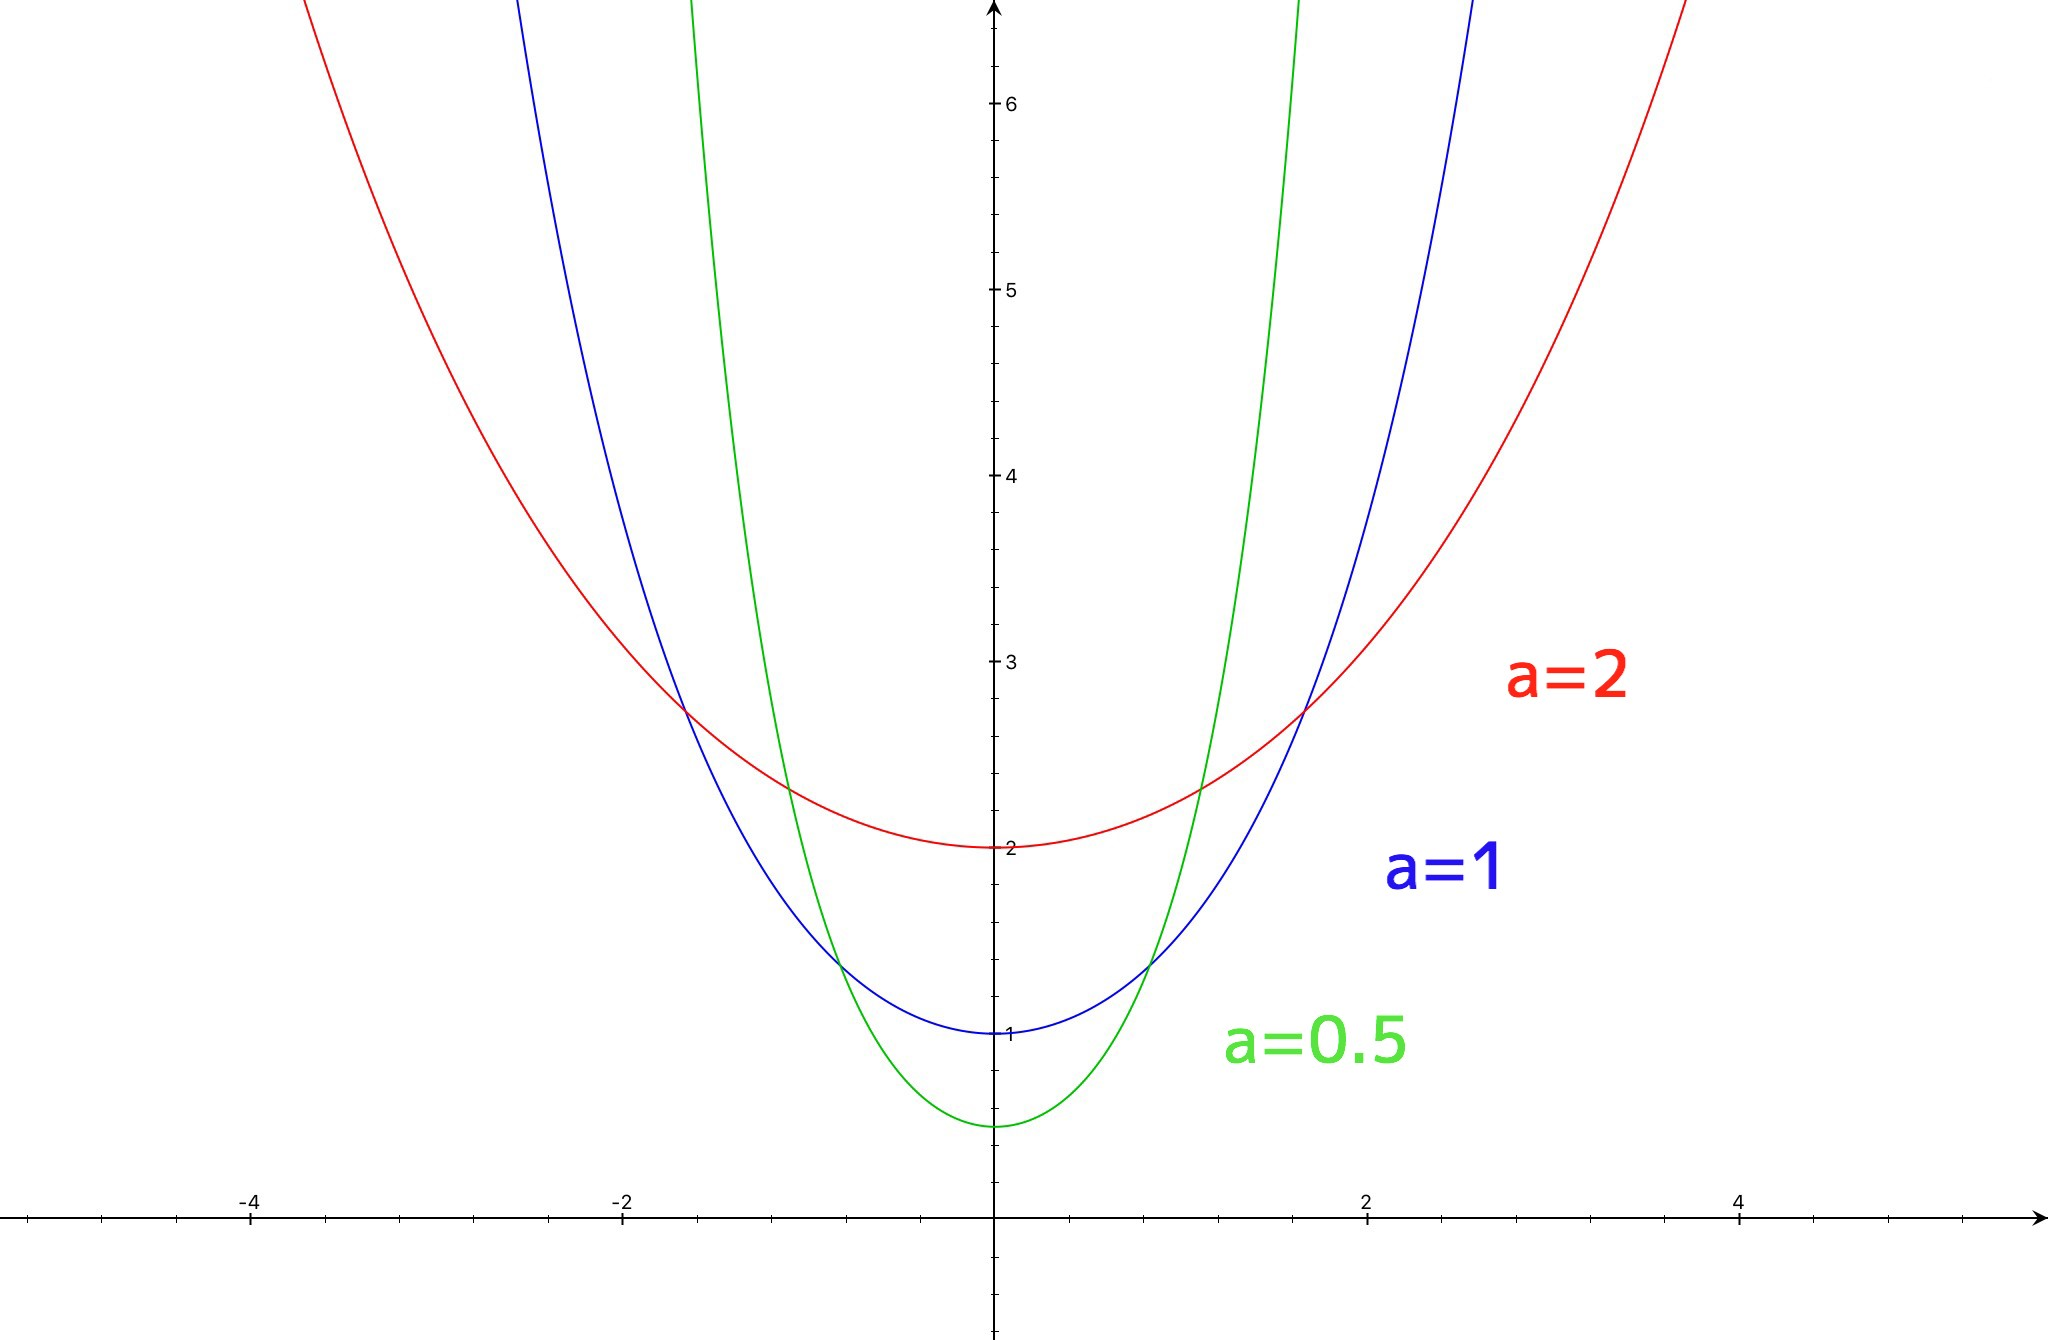
\includegraphics[width = 11cm]{nakayama/image/catenary1.JPG}
\end{center}


\newpage
\section{曲線の長さ}
\subsection{積分計算}

カテナリー曲線は$y = a\cosh{\frac{x}{a}}$で表せることがわかった。頂点の座標は$(0,a)$である。

それでは曲線の長さ$L$を求めよう。径間距離(ひもを支える2点間の距離)を$D$とすると
\begin{eqnarray*}
L & = & \int_{-D}^D ds \\
& = & 2 \int_0^\frac{D}{2} ds \\
& = & 2 \int_0^\frac{D}{2} \sqrt{dx^2 + dy^2} \\
& = & 2 \int_0^\frac{D}{2} \sqrt{1 + \left(\frac{dy}{dx}\right)^2}\,\,dx \\
& = & 2 \int_0^\frac{D}{2} \sqrt{1 + \sinh^2\frac{x}{a}}\,\,dx \\
& = & 2 \int_0^\frac{D}{2} \cosh \frac{x}{a}\,\,dx \\
& = & 2 \left[a\sinh \frac{x}{a}\right]_0^\frac{D}{2} \\
& = & 2a\sinh\frac{D}{2a} \\
& = & 2a\cdot\frac{\, e^{\frac{D}{2a}} - e^{-\frac{D}{2a}}}{2}
\end{eqnarray*}\par
指数関数をテイラー展開して
\begin{eqnarray*}
\qquad\qquad\qquad\quad & = & a\left(\sum_{k = 0}^\infty \frac{1}{k!}\left(\frac{D}{2a}\right)^k - \sum_{k = 0}^\infty \frac{1}{k!}\left(-\frac{D}{2a}\right)^k\right)
\end{eqnarray*}\par
$k = 2j + 1$(奇数)の項だけ残って
\begin{eqnarray*}
\qquad & = & 2a\sum_{j = 0}^\infty \frac{1}{(2j + 1)!}\left(\frac{D}{2a}\right)^{2j + 1}
\end{eqnarray*}\par
$j$を改めて$k$とおいて整理すると
\begin{eqnarray*}
& = & \sum_{k = 0}^\infty \frac{D^{2k + 1}}{(2a)^{2k}(2k + 1)!}. \quad
\end{eqnarray*}

これで$L$を級数で表すことができた。

\subsection{具体的な数値}
$\displaystyle L = \sum_{k = 0}^n \frac{D^{2k + 1}}{(2a)^{2k}(2k + 1)!}$で近似を計算した。表の値は小数点以下7桁目を四捨五入している。\\\par
$D = 2$のとき
\begin{table}[htb]
\begin{center}
\begin{tabular}{cc}

\begin{minipage}{0.5\hsize}
\begin{center}
a = 0.5 \\
\begin{tabular}{c|c} \hline
n & L \\ \hline
1 & 3.333333 \\
2 & 3.600000 \\
3 & 3.625397 \\
4 & 3.626808 \\
5 & 3.626859 \\ \hline
正確な値 & 3.62686040784... \\ \hline
\end{tabular}
\end{center}
\end{minipage}

\end{tabular}
\end{center}
\end{table}


\begin{table}[htb]
\begin{center}
\begin{tabular}{cc}

\begin{minipage}{0.5\hsize}
\begin{center}
a = 1 \\
\begin{tabular}{c|c} \hline
n & L \\ \hline
1 & 2.333333 \\
2 & 2.350000 \\
3 & 2.350397 \\
4 & 2.350402 \\ \hline
正確な値 & 2.35040238728... \\ \hline
\end{tabular}
\end{center}
\end{minipage}

\begin{minipage}{0.5\hsize}
\begin{center}
a = 2 \\
\begin{tabular}{c|c} \hline
n & L \\ \hline
1 & 2.083333 \\
2 & 2.084375 \\
3 & 2.084381 \\
4 & 2.084381 \\ \hline
正確な値 & 2.08438122197... \\ \hline
\end{tabular}
\end{center}
\end{minipage}

\end{tabular}
\end{center}
\end{table}

\clearpage
$D = 5$のとき

\begin{table}[htb]
\begin{center}
\begin{tabular}{cc}

\begin{minipage}{0.5\hsize}
\begin{center}
a = 0.5 \\
\begin{tabular}{c|c} \hline
n & L \\ \hline
1 & 25.833333 \\
2 & 51.875000 \\
3 & 67.375992 \\
4 & 72.758281 \\
5 & 73.981528 \\
6 & 74.177562 \\ \hline
正確な値 & 74.203210577788... \\ \hline
\end{tabular}
\end{center}
\end{minipage}

\end{tabular}
\end{center}
\end{table}

%
\begin{table}[htb]
\begin{center}
\begin{tabular}{cc}
%
\begin{minipage}{0.5\hsize}
\begin{center}
a = 1 \\
\begin{tabular}{c|c} \hline
n & L \\ \hline
1 & 10.208333 \\
2 & 11.835938 \\
3 & 12.078141 \\
4 & 12.099165 \\
5 & 12.100360 \\ \hline
正確な値 & 12.1004089620... \\ \hline
\end{tabular}
\end{center}
\end{minipage}
%
\begin{minipage}{0.5\hsize}
\begin{center}
a = 2 \\
\begin{tabular}{c|c} \hline
n & L \\ \hline
1 & 6.302083 \\
2 & 6.403809 \\
3 & 6.407593 \\
4 & 6.407675 \\
5 & 6.407676 \\ \hline
正確な値 & 6.40767632120... \\ \hline
\end{tabular}
\end{center}
\end{minipage}
%
\end{tabular}
\end{center}
\end{table}
%
\section*{参考文献}
\begin{enumerate}
  \item	吉田武,『新装版 オイラーの贈物』(東海大出版部,2015)
  \item \url{http://mathtrain.jp/int_sinnx},『sinのn乗,cosのn乗の積分公式』
  \item \url{https://ja.wikipedia.org/wiki/楕円積分}
  \item \url{https://ja.wikipedia.org/wiki/カテナリー曲線}
  \item \url{http://mathtrain.jp/catenary},『懸垂線の2通りの導出』
\end{enumerate}
 \clearpage



\chapter*{}
\vspace{10zw} % 高さ調整
\begin{center}
  \textgt{
    {\Huge 第III部} \\ \vspace{15pt}
    {\Huge 共鳴を物理的に考察してみる} \\ \vspace{20pt}
    {\Large 理工学部 物理科学科} \\ \vspace{5pt}
    {\Large  門野広大} \vspace{40pt}
    }
\end{center}
\addcontentsline{toc}{part}{第III部 共鳴を物理的に考察してみる \\ \hspace{4zw}{\small 理工学部 物理科学科 門野 広大 }}
\clearpage

\section*{数学と物理の関係}
物理と数学は高校までは別物として授業を行っているが、ちゃんと物理をしていくと物理と数学の違いがわからなくなるくらいに物理では数学をよく使っている。私が思うに数学は自然現象を記述していくための言語である。自然現象自体にもともと名前がついているわけはないし取扱説明書があるわけはない。でも人間は自然現象を理解していくためには言語化しないといけない。だけども日本語とか英語とかで自然現象を記述するのは難しいしきっと莫大な量になってしまう。そこで登場してくるのが数学である。数学を使用するととても簡単に記述することができてしまうし数学はどの国に行っても記述の方法は一緒なので翻訳する必要はない。といったことで物理では数学は必須言語なのである。
\section*{この文の構成}
本当はもう少し簡単なところから書いていこうかとも思ったのですが、時間などの関係上その部分はなくなってしまいました。そのため簡単な数学や力学をかじってないと結構専門的な文章になっていると思うので物理をまったくやってない人は共鳴というものを説明するにはこんなにも数学を使うんだなあと思うくらいで目を通してくださると幸いです。



\newpage

\chapter{強制振動~共鳴まで}
\section{減衰振動}
今回は共鳴というものを数式的にどのようにわかるかということを示してみる。\\
まず、抵抗力の働いたばねの振動を考える。この振動の運動の運動方程式は、
\begin{eqnarray}
m\frac{d^2x}{dt^2}+b \frac{dx}{dt} + kx&=&0 \\
\frac{d^2x}{dt^2}+2\gamma \frac{dx}{dt} + {\omega_0}^2 x&=&0\\
\left(\gamma = \frac{b}{2m} ,  {\omega_0}^2  = \frac{k}{m} \right) \nonumber
\end{eqnarray}

で表すことができる。この微分方程式は二階の同次線形微分方程式である。この微分方程式の一般解を求める。$x=e^{\lambda t}$とおいて式(2)に代入すると、
\begin{eqnarray}
{\lambda}^2+2\gamma \lambda+{\omega_0}^2 = 0 \nonumber \\
\lambda = -\gamma \pm \sqrt{{\gamma}^2-{\omega_0}^2}
\end{eqnarray}
となる。よってこの$\lambda$の解は三つの場合に分けることができる。場合分けを行って式(2)の一般解を求める。\\
(1)$\omega_0 < \gamma$つまり復元力よりも抵抗力が大きい時を考える。この条件では$\lambda$が実数値を持つよって式(2)解の重ね合わせで表現できるので
\begin{eqnarray}
x(t)&=&C_1e^{-\gamma t}e^{\sqrt{{\gamma}^2-{\omega_0}^2}t}+C_2e^{-\gamma t}e^{-\sqrt{{\gamma}^2-{\omega_0}^2}t}
\end{eqnarray}
という形で表される。この式の振幅はすぐに減衰してしまい振動しない(過減衰)\\
\begin{figure}[H]
\centering
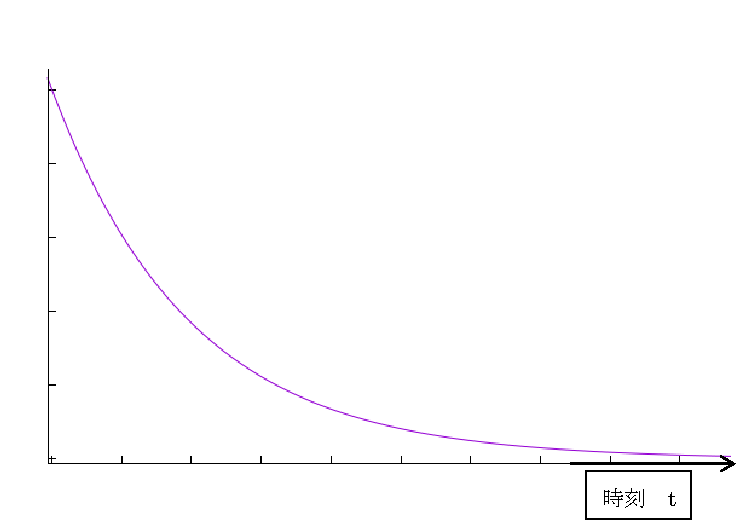
\includegraphics[height=7cm,clip]{kadono/image/gensui.pdf}
\label{fig:ele1}
\caption{過減衰}
\end{figure}
(2)$\omega_0 = \gamma$つまり$\lambda$が重根を持つとき、解が一つしか持たない、よって変数変化法を用いてこの場合の一般解を求めると、
\begin{eqnarray}
x(t)&=(At+B)e^{-\gamma t}
\end{eqnarray}
となる。この場合も同じように指数関数的に減衰する。(臨界減衰)\\
(3)$\omega_0 > \gamma$つまり抵抗力が小さい時を考える。この条件では$\lambda$が虚数となる。よって式(3)の$\lambda$の解を書き換えると
\[
\lambda = \pm i\omega - \gamma  \ \ \ \ \ \ \  (\omega= \sqrt{\omega^2-\gamma^2})
\]
とすると、(1)と同じように表すことができる。
\begin{eqnarray}
x(t)	&=&C_1e^{-\gamma t}e^{-i\omega t}+C_2e^{-\gamma t}e^{+i\omega t} \nonumber\\
	&=&e^{-\gamma t}(C_1e^{-i\omega t}+C_2e^{+i\omega t})\nonumber\\
	&=&Ce^{-\gamma t}\cos (\omega t +\phi)
\end{eqnarray}
となる。この振動は単振動のような振動しながら振幅は指数関数的に徐々に減少していく。(減衰振動)
\begin{figure}[H]
\centering
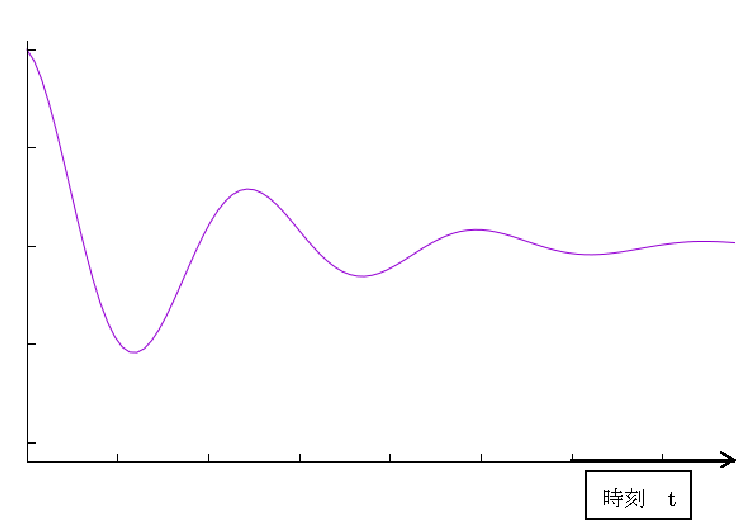
\includegraphics[height=7cm,clip]{kadono/image/gensui1.pdf}
\label{fig:ele1}
\caption{減衰振動}
\end{figure}


\section{強制振動}
強制振動とは、外部から周期的に力を加えられることによって振動する振動を強制振動という。式(1)に外部からの力の項を加えると
\begin{eqnarray}
m\frac{d^2x}{dt^2}+b \frac{dx}{dt} + kx&=& F(t)
\end{eqnarray}
となる。ここで$F(t)=F_0\cos {\omega t}$という形の微分方程式を考える。

\begin{eqnarray}
\frac{d^2x}{dt^2}+2\gamma \frac{dx}{dt} + {\omega_0}^2 x&=&f\cos{\omega t}\ \ \ \ \ (f = F_0/m)
\end{eqnarray}
となる。この微分方程式は非同次微分方程式である。このような微分方程式の一般解は同次の一般解と非同次の特解の和で求められることが知られている。なぜかは数学の得意な人に聞いて下さい。\\
同次の一般解はもう求めてあるので、必要なのは(8)の特解である。しかしなかなかこの微分方程式は求まらないので虚数の項を加えてみたらうまくいくらしいので、そうしてみる。よって(8)の右辺に
\[
if\sin{\omega t}
\]
を加えてみるそうすると
\begin{eqnarray}
\frac{d^2x}{dt^2}+2\gamma \frac{dx}{dt} + {\omega_0}^2 x&=&fe^{i\omega t}
\end{eqnarray}
となる。これだとうまくいきそうなのでこれをこれで特解を求めてみることにする。まず特解を
\begin{eqnarray}
x_s = Ae^{i\omega t}
\end{eqnarray}
と仮定して(9)に入れてみると....
\begin{eqnarray}
(-\omega^2 +2\gamma \omega i + {\omega_0}^2)Ae^{i\omega t}=fe^{i\omega t}
\end{eqnarray}
となりこれを$A$について解くと、
\begin{eqnarray}
A=\frac{f}{\sqrt{({\omega_0}^2-\omega^2)^2+4\gamma^2\omega^2}}e^{i\psi}
\end{eqnarray}
となる。これで(9)の特解を求めることができる。
\begin{eqnarray}
x_s = \frac{f}{\sqrt{({\omega_0}^2-\omega^2)^2+4\gamma^2\omega^2}}e^{i\omega t +\psi}
\end{eqnarray}
となる。でも私たちが知りたいのは(8)の特解である。これは、(13)の実数部分がそのものである。なぜそうなるかは考えてみると結構早くわかるが、簡単に言うと複素数を微分するとき、実数部分の微分に虚数の部分の微分がかかわってくることがないからである。\\
よって、式(8)の特解は
\begin{eqnarray}
x_s = \frac{f}{\sqrt{({\omega_0}^2-\omega^2)^2+4\gamma^2\omega^2}}\cos(\omega t +\psi)
\label{eq:tokkai}
\end{eqnarray}
よって求まった!
\section{ここから何が分かるのか}
ようやく強制振動の運動方程式の一般解が求まったですが、そもそもここから何が読み取れるのか何が分かるのかをわからないと意味がない、\\
前の部分では、正直言うと強制振動の特解しか求めていない、これには理由が存在している。それは、非斉次の微分方程式の特解は斉次の一般解と特解との和で表せる。という話であった。ここで斉次の一般解とはそもそも減衰していってしまうものであり、それはいつかなくなってしまう項である。そんな未来性のない項を考えても仕方がないというのでじゃあ特解だけでいいやということで特解だけをあえて残した。\\
特解(\ref{eq:tokkai})の式は基本の形は単振動の式である。外力で変えられるものは
\[
f , \omega
\]
である。でも$f$を変えてもただ単調に増えていくだけでそこまで特徴を見出せない。では$\omega$はを変えていくとどのように変化していくのかを考えてみるとある特徴的な現象を説明することができる。まずは特解(\ref{eq:tokkai})の式の形について考えてみる。この特解の形を簡単に記号に置き換えて考えてみると
\begin{eqnarray}
  x_s = A\cos(\omega t + \psi)  \left(A = \frac{f}{\sqrt{({\omega_0}^2-\omega^2)^2+4\gamma^2\omega^2}} \right)
\end{eqnarray}
という形であることが分かる。この形は単振動の式とまったく変わらない。$A$は本当にただの振幅なのかどうかが気になるひとがいるだろう。しかしただの振幅である。$A$で使ってる変数は$\omega_0\ \omega \ \gamma \  f$である。一つ一つ見ていくと$\omega_0$は減衰振動の振動数であるので時間に依存しない変数である。$\gamma$は上で定数として定義していたので時間によって変化されてしまったら困る。$\omega ,\ f$は前で述べたように外力の振動数のその大きさであるのでこれも時間に依存してしまったらとても難しい運動になってしまうのでひとまず時間に依存しない変数とする。\\
以上より、ここで特解は上の式で表すことができることが分かった。ここでようやく$\omega$を変えることによってどんな面白いことがあるかを考えて見ることにします。$\omega$を変えると特解のどこが変化するかというと上の式の$A$であるつまり単振動の振幅の値である。振幅の値が変化するということはその振動が大きくなるということである。振幅が大きくなるとその運動を人間が見やすくなるということである。そのほかにも波のエネルギーは振幅の二乗で求めることができることが知られていてつまり振幅が大きくなるとその波のエネルギーは大きくなっていく。このエネルギーの源は何だったかを考えると、外力である。特解の振幅が大きいほど外力のエネルギーを効率よく波が吸収しているということである。この現象を共鳴という。\\
$\omega$がどのようになったら振幅の値が大きくなるのかを考える。$A$が最大になるためには$A$の分母が最小になるときなのでその時は$\omega = \omega_0$の時である。ここで$\gamma<\omega_0$であることに注意すると簡単に求めることができる。\\
この$\omega$計算的にもとめることはここでできた。しかし、実際はこの$\omega$を実験で求める必要がある。ここで$Aを\omega$の関数としてグラフを作成してみると下図のようになる。
\begin{figure}[H]
\centering
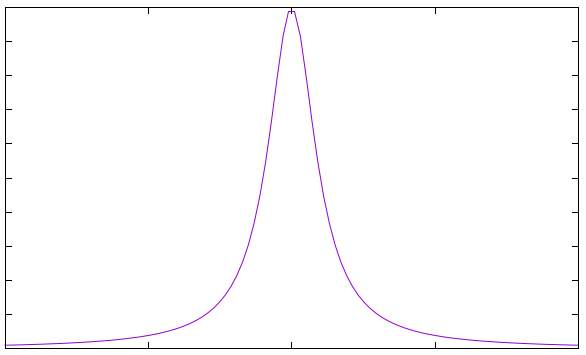
\includegraphics[height=7cm,clip]{kadono/image/reso.png}
\label{fig:reso}
\caption{共鳴曲線}
\end{figure}

\newpage

\chapter{共鳴現象を利用した実験例}
ここまで共鳴現象というものを理論的に数学的に記述してきた。この現象がいったいどのくらい物理の実験や現実世界で使われいるのかの一例をここから書いていきたいと思います。\\
ここから書いてあるものは実際に私が実験したものを抜粋してきたものになっています。概要を見たら大体実験の内容が分かるかと思いますが、簡潔に言うとLC回路が共鳴するときの振動数を図ってコイルの自己インダクタンスを求めようということです。
\begin{center}
\section*{LC回路を使用した自己インダクタンスの測定}
\end{center}
\subsection*{概要}
ICカードに使われている電気回路に注目して実験を行った。ICカードの中にはLC直列回路が入っておりその回路が共鳴現象を起こすことによって電力が供給されている。今回の実験はこのICカードに利用されている電気回路をなるべく再現しLC直列回路に共鳴現象が起きることを確認しその実験のデータからコイルの自己インダクタンスを求めた。結果として今回作製したコイルの自己インダクタンスは$7.5\times 10^{-5}\ {\rm H}$であることが分かった。


\section{序論}
今日では従来必需品であったものがどんどんなくなってきている。その中の一つは現金である。今では電車に乗るときはICOKAやSUIKAなどのICカードを使用しいる。ICカードは今やいろんなところで使用されているが、このカードの特徴は機器にかざすだけで商品の支払いが終わる。カードと機器の間はもちろんだがつながってはいない、加えてカードのほうには電力原が存在していない。どうしてこんなただカードで情報のやり取りができるのか、どうして電力原がないカードに電流が通るのかこの疑問について考えていきたいと思う。ICカードには電気回路が入っている。この回路簡単に言うとLC直列回路である。この中には電源がないのにこの回路が動作するのかを説明するのにLCR直列回路の共鳴現象について説明たいと思う。いま考えるLCR直列回路は図\ref{fig:ele}の(A)に示す。この回路で時刻をt、コイルの自己インダクタンスをL、抵抗をR、コンデンサの電気容量をC、交流電圧を$V_0 \cos{\omega t}$、回路の中を流れる電流を$i$とするとこの電気回路の微分方程式を次に示す。
\begin{eqnarray}
L\frac{d^2i}{dt^2}+R\frac{di}{dt}+\frac{i}{C}=V_0\cos{\omega t}
\end{eqnarray}
この式の特解は
\begin{eqnarray}
i=I\sin(\omega t + \phi)\ \ \ \ \ \left(I=\frac{V_0}{\sqrt{R^2+(\omega L- \frac{1}{\omega C})^2}}\right)
\end{eqnarray}
となる。ここで振幅が最大になるような$\omega $は$I$の分母の値が最小になるときなので
\begin{eqnarray}
\omega =\omega_0=\frac{1}{\sqrt{LC}}=\frac{1}{\sqrt{L}}C^\frac{1}{2}
\end{eqnarray}
となる。\\
以上よりLCR直列回路にある特定の周波数の電圧を加えると電流の値が最大の値をとることが分かった。この関係をグラフにすると図\ref{fig:ele}の(B)のようになる。ここで
\[
Q=\frac{\omega_0}{\omega_2-\omega_1}
\]
と定義されている共鳴の鋭さというものがある。$\omega_1,\omega_2$はそれぞれ$V_m/\sqrt{2}$の値をとるときの各振動数である。このQ値というのは図\ref{fig:ele}の(C)の共鳴振動数の周辺の鋭さを示す物である。このQ値が示す物理的な意味はどれだけエネルギーを安定的に吸収したかを表すものである。

以上で電気回路の共鳴現象については理論的には分かった。ここでICカードには電力源がないのにどのように電力を供給しているのかを考える。コイルは時間的に磁場が変化する空間に置かれるとあるその磁場の変化に対応した電圧が生じる。この現象は発電システムにも利用されている。この現象を利用してICカードに電力が供給されている。この現象を利用した共鳴回路を図\ref{fig:ele}の(C)に示す。今回の実験はこの現象を利用しLC直列回路に電力を供給し共鳴現象を起こした。\\
数式(3)からわかるように固有角振動数は電気容量の-1/2倍に比例することが分かる。今回の実験はコイルの自己インダクタンスを求めることを目的とし固有振動数と電気容量の間の関係を調べた。
\\
\begin{figure}[H]
\centering
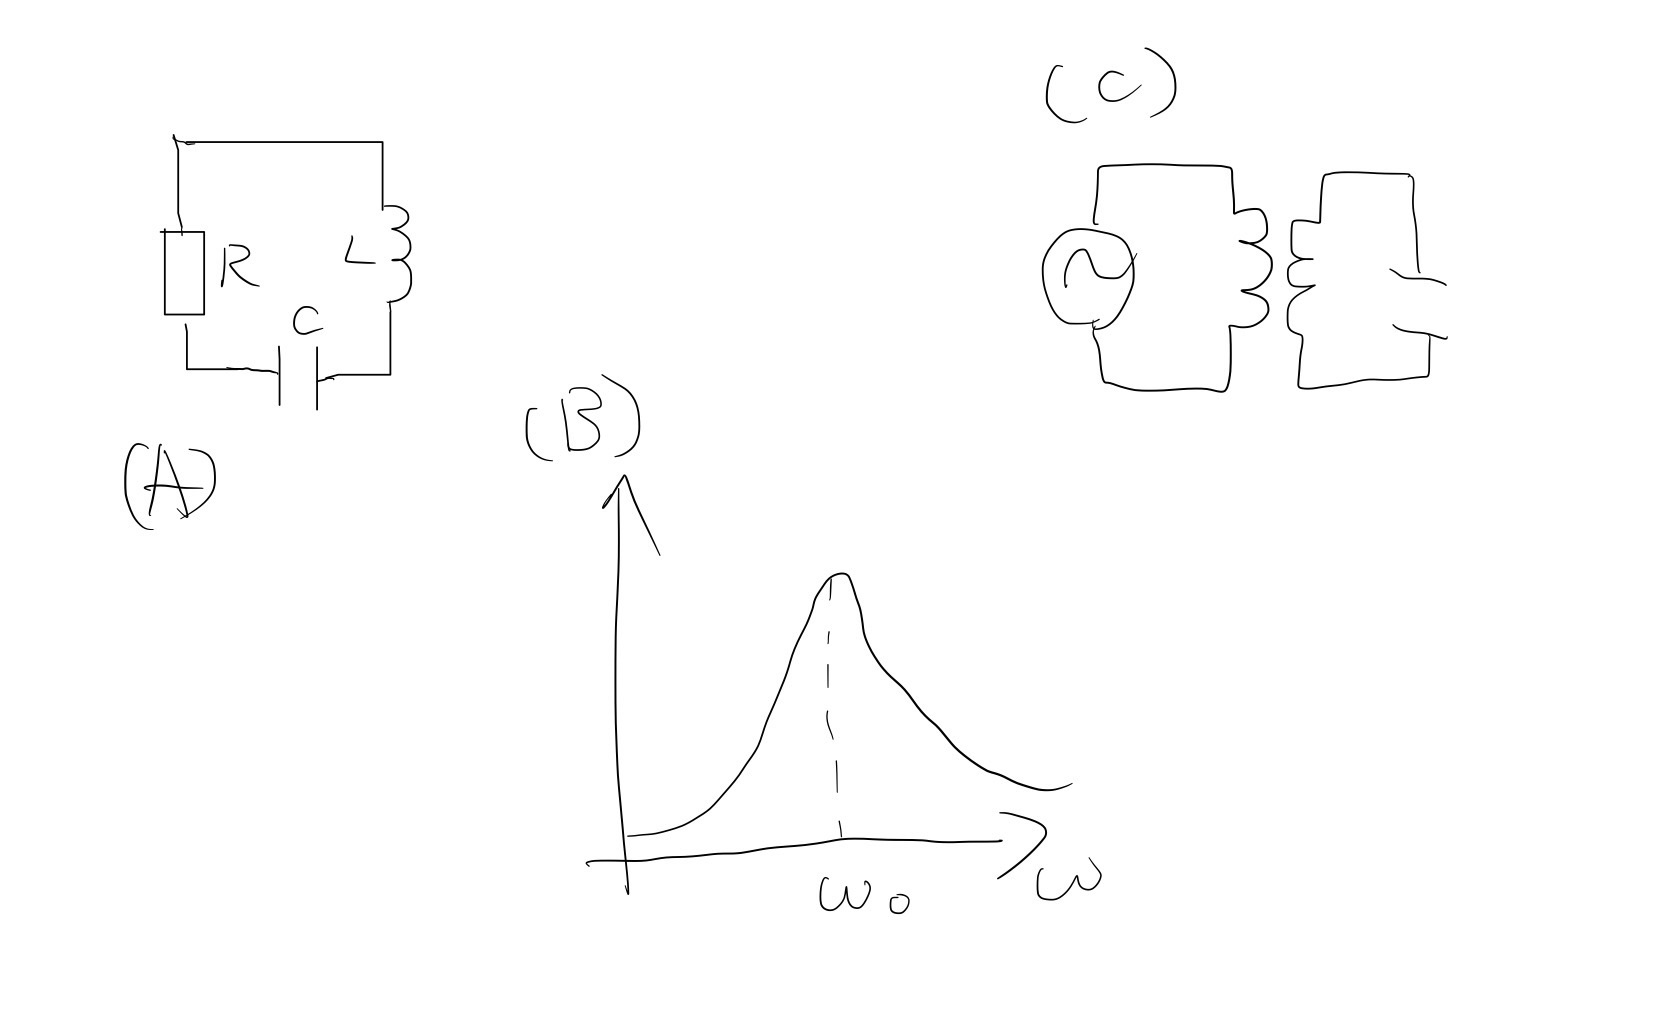
\includegraphics[height=8cm,clip]{kadono/image/houhou.jpg}
\label{fig:ele}
\caption{(A):LCR直列回路、(B)振動数と振幅との関係のグラフ、(C):コイルを使用して電力を供給したLC直列回路}
\end{figure}
\newpage
 \section{実験方法}
今回行った実験の模式図を図\ref{fig:ele1}に示す。回路図上のコイル部分はアクリル製のパイプ(外形21 mm内径18 mm)に0.4 mmの被覆銅線を使用した。一次コイル(ファンクションジェネレーターにつながっている方)に30回巻き、二次コイル(コンデンサにつながっている方)を90回巻きにして一次コイルと二次コイルは同じパイプ上に間を開けて巻いた。(このときコイルに巻いた銅線のはじめと終わりをやすりなどでこすり表面の被覆を落とし電流が通るようにする)\\
 コンデンサを図のようにつなげファンクションジェネレータによって一次コイルにかかる振動数を変えて振幅の値が最大になる振動数(共鳴振動数)を探した。見つけた共鳴振動数の$\pm 0.1$MHzの範囲で$0.01$MHz刻みでオシロスコープから振幅の値を読みとった。共鳴振動数での周辺で振動数と振幅のデータが20個を得られた。このデータを使用して横軸に振動数、縦軸に振幅をとったグラフ(共鳴曲線)を書き、このデータから共鳴の鋭さ(Q値)を求めた。コンデンサの電気容量を変化させて再度共鳴振動数での周辺の振動数と振幅のデータをとりそのデータからQ値を求めた。各電気容量での共鳴振動数を求めたのち電気容量と共鳴振動数の関係のグラフを書きそのグラフから今回使用した自己インダクタンスを求めた。

\begin{figure}[H]
\centering
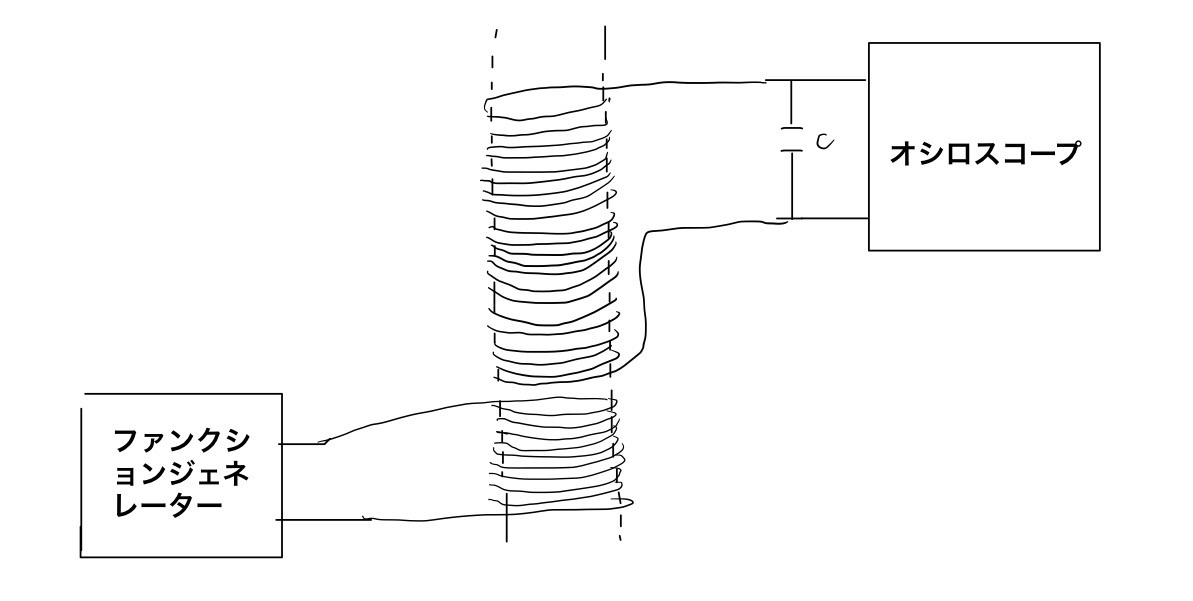
\includegraphics[height=5cm,clip]{kadono/image/houhou2.jpg}
\label{fig:ele1}
\caption{コイルの電磁誘導を使用したLC共鳴回路の模式図}
\end{figure}







\newpage
 \section{実験結果}
コンデンサの電気容量はLCRメータを用いて測定した値である。具体的なデータの値は付録を参照\\
電気容量45.8 pFの時の周波数と振幅の値の関係のグラフを次に示す。
\begin{figure}[H]
\centering
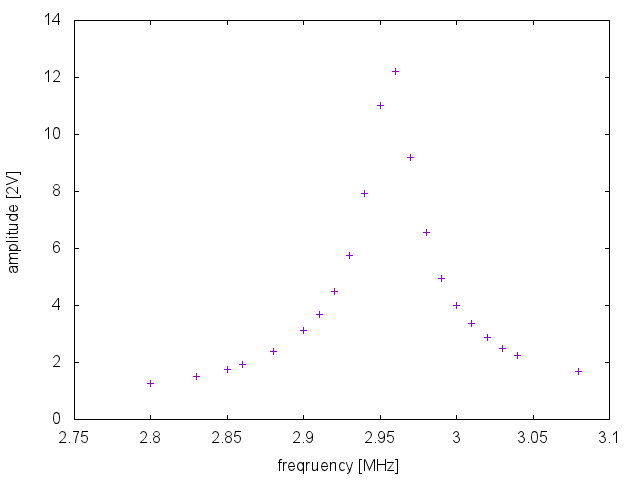
\includegraphics[height=7cm,clip]{kadono/image/45_8.png}
\label{fig:45.8}
\caption{45.8pFでの振動数[MHz]と振幅[V]の共鳴曲線}
\end{figure}
このときの共鳴振動数とその時の振幅$V_m$をグラフから読むと
\[
f_0=2.96\ {\rm MHz}\ \ \ V_m = 6.1\ {\rm V}
\]
であり、そのとき$V_m/\sqrt{2}$の値をとる振動数$f_1,f_2$は、データより
\[
f_1\sim 2.94\ {\rm MHz}\ \ \ f_2 \sim 2.975\ {\rm MHz}
\]
なので共鳴の鋭さQ値は
\[
Q=\frac{f_0}{f_2-f_1}\sim84.5
\]
となる。

他の電気容量の場合も45.8 pFの時と同様にして$f_0 , V_m , f_1 , f_2 , Q$を求める。その値を次の表に示す。各電気容量での振動数と振幅の関係のグラフは付録を参照
\begin{table}[H]
\caption{各電気容量の共鳴曲線から読み取れる値}
\centering
\begin{tabular}{c|c|c|c|c|c}
電気容量[pF]	&固有振動数$f_0$[MHz]	&最大振幅$V_m$[V]		&$f_1$[MHz]	&$f_2$[MHz]	&Q\\ \hline
45.8			&2.96					&6.1						&2.94		&2.975		&84.5\\
195.4		&1.49					&12.5					&1.44		&1.545		&14.2\\
292.0		&1.24					&12.4					&1.20		&1.285		&14.6\\
443.8		&1.00					&11.5					&0.97		&1.04		&14.3\\
663.0		&0.84					&17.7					&0.815		&0.855		&21.0\\\hline
\end{tabular}
\end{table}
上の表から電気容量が上がっていくにつれて共鳴振動数が減少していくことが分かる。この関係を図4に示す。\\
\begin{figure}[H]
\centering
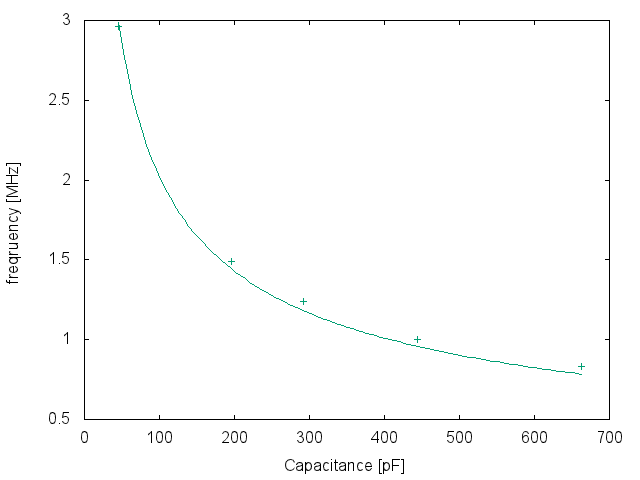
\includegraphics[height=8cm,clip]{kadono/image/all.png}
\label{fig:real}
\caption{共鳴振動数と電気容量の関係のグラフ}
\end{figure}
このグラフの線は各点が滑らかに引けると仮定して引いた線である。ここで理論によって導きだした式(3)と$f=\omega /2\pi$という関係より
\begin{eqnarray}
f_0=\frac{1}{2\pi \sqrt{LC}}
\end{eqnarray}
という関係式が導きだされる。この理論による数式と図4の曲線がどのくらい一致するか確認するために次に両対数のグラフを示した。
\begin{figure}[H]
\centering
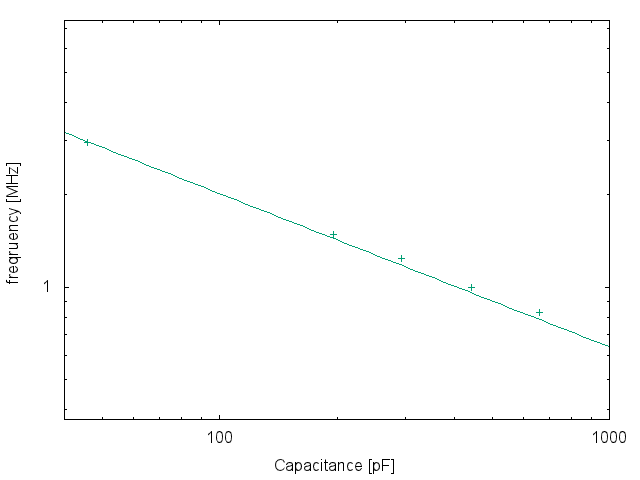
\includegraphics[height=8cm,clip]{kadono/image/f-clog.png}
\label{fig:logsc}
\caption{共鳴振動数と電気容量の関係の両対数グラフ}
\end{figure}
このグラフの線は各点のなるべく近くを通るように引いた線である。ここで最小二乗法を用いてこの線の傾きを求めると-0.48である。これはほとんど-1/2であるので共鳴振動数は電気容量の-1/2乗に比例することが確認された。\\
ここから自己インダクタンスLを求めることができることができるはずである。上記の共鳴振動数を求める数式(4)の両辺に対数をとると
\begin{eqnarray}
\log f_0= -\frac{1}{2}\log{C} + \log{\frac{1}{2 \pi \sqrt{L}}}
\end{eqnarray}
となる。ここで最小二乗法で求めた図5の切片は1.26であるので上の数式から今回作製したコイルの自己インダクタンスを求めると
\begin{eqnarray}
L=7.54 \times 10^{-5} {\rm H}
\end{eqnarray}
となる。







 \section{考察}
求めたQ値について評価すると、Qの値は電気容量が上がっていっても一定の変化をしているようには表1からは読み取れない。Q値が最大の値をとっている45.8pFの時の共鳴曲線と最小の値をとっている195.4pFの共鳴曲線を見比べてみると共鳴振動数の周辺での勾配が45.8pFの時のほうが大きくなっている。序論で言った通りQ値の値は共鳴の鋭さでありどれだけ効率よくエネルギーを吸収しているのかを示している値である。よって今回の実験の結果から45.8pFの時には安定してエネルギーが吸収されたことが分かる。しかし、45.8pFの以外の電気容量でのQ値はほとんど値が同じくらいである。Q値は
\[
Q=\frac{\omega_0}{\Delta \omega}=\frac{1}{\omega_0 RC}
\]
とも書き表せる。[3]この式から電気容量が増加するとQ値は減少するはずである。この結果は今回の実験と反している。今回の実験では45.8pFの時を測定して間を空けてほかの場合を測定してしていてその時にいろんな条件が変化してしまい何かノイズが生じてしまい振幅の値を誤って測定してしまった可能性がある。


次に今回の実験で求めた自己インダクタンスの値について別の視点から求めその値とどのくらい一致するのかを考察する。コイルの巻き数N, 断面積S, 長さlの自己インダクタンスは
\begin{eqnarray}
L=\frac{\mu_0 N^2 S}{l}
\end{eqnarray}
という関係式で求めることができる($\mu_0$は真空の透磁率)。[4] この関係を用いて今回使用したコイルのインダクタンスを求めると
\begin{eqnarray}
L = \frac{90^2 \times 10.5^2 \times \pi \times 10^{-3}\times \mu_0 }{0.4 \times 90 \times 10^{-3}}= 9.8 \times 10^{-5}\ \ [{\rm H}]
\end{eqnarray}
となる。ここで計算したコイルのインダクタンスの値は隙間ないく巻いているという条件で計算したものである、しかし今回作製したコイルはかなり簡易的なものでありところどころ隙間が目視できる状態であった。この点を考慮して(6)と(8)の値を比較するとほとんど同じような値であることが分かる。よって今回作成したコイルの自己インダクタンスは(6)の値であることが確認された。













 \section{結論}
今回使用したコイルの自己インダクタンスは$7.54\times10^{-5}$[H]であることが分かった。

\section*{参考文献}
\begin{enumerate}
  \item	兵頭俊夫著 考える力学 学術図書出版社
  \item 小形正男著 振動・波動 裳華房
  \item 宇田川眞行他編  物理学基礎実験 (第2版新訂) 共立出版株式会社 2012.
  \item 佐川弘幸・本間道雄著 物理学スーパーラーニングシリーズ 電磁気学 丸善出版 1997
  \item 小形正男著 振動・波動 (第11版) 裳華房 2008
\end{enumerate}

\section*{A付録 共鳴曲線}

\begin{figure}[H]
\centering
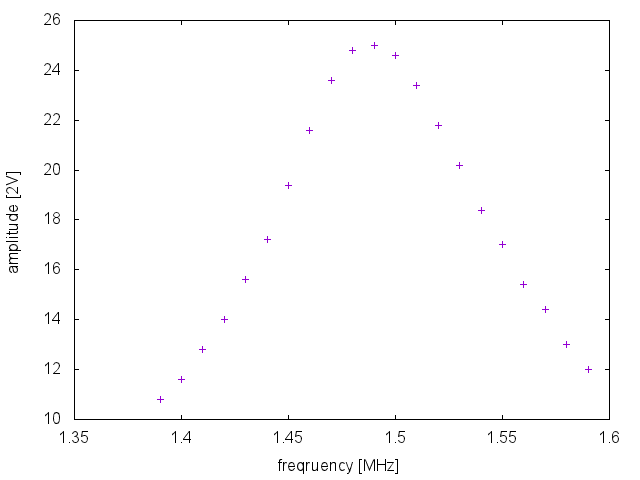
\includegraphics[height=5cm,clip]{kadono/image/195.png}
\label{fig:195.4}
\caption{195.4pFでの振動数[MHz]と振幅[V]の共鳴曲線}
\end{figure}
\begin{figure}[H]
\centering
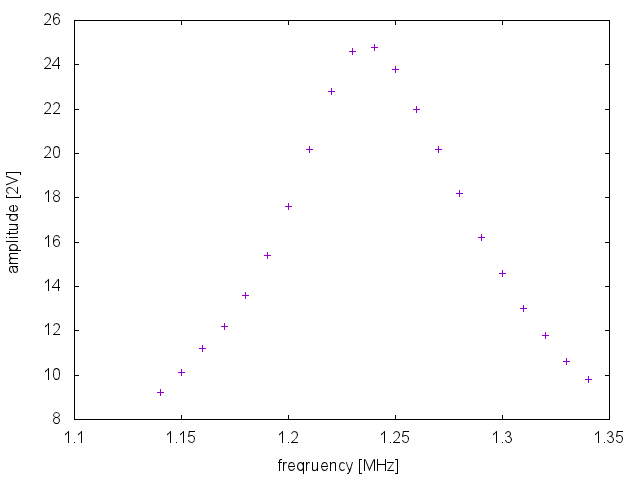
\includegraphics[height=5cm,clip]{kadono/image/292.png}
\label{fig:292.0}
\caption{292.0pFでの振動数[MHz]と振幅[V]の共鳴曲線}
\end{figure}
\begin{figure}[H]
\centering
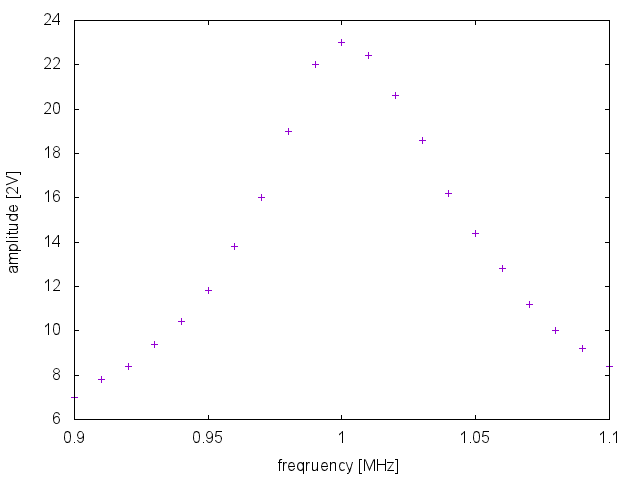
\includegraphics[height=5cm,clip]{kadono/image/443.png}
\label{fig:443.8}
\caption{443.8pFでの振動数[MHz]と振幅[V]の共鳴曲線}
\end{figure}
\begin{figure}[H]
\centering
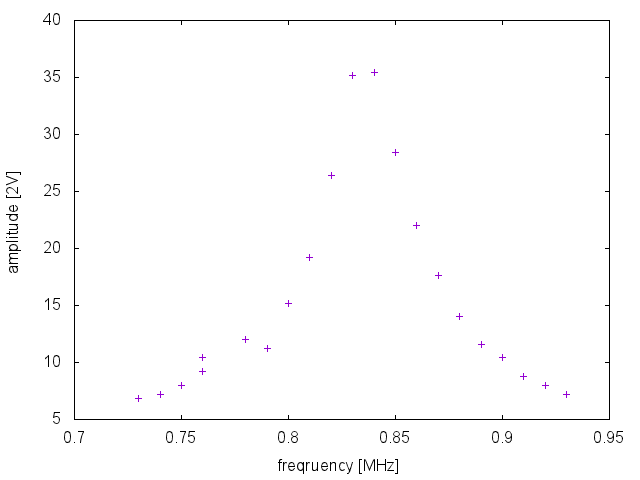
\includegraphics[height=5cm,clip]{kadono/image/663.png}
\label{fig:663}
\caption{663.0pFでの振動数[MHz]と振幅[V]の共鳴曲線}
\end{figure}
 \clearpage


\chapter*{}
\vspace{10zw} % 高さ調整
\begin{center}
  \textgt{
    {\Huge 第IV部} \\ \vspace{15pt}
    {\Huge 自家製ロケットエンジン\\(Homemade Rocket Engine)} \\ \vspace{20pt}
    {\Large 理工学部 電気電子工学科} \\ \vspace{5pt}
    {\Large  岡田 優人} \vspace{40pt}
    }
\end{center}
\addcontentsline{toc}{part}{第IV部 自家製ロケットエンジン(Homemade Rocket Engine) \\ \hspace{4zw}{\small 理工学部 電気電子工学科 岡田 優人 }}
\chapter{自家製ロケットエンジン(Homemade Rocket Engine)}
\section{目的}
固体ロケット推進剤を理解するとともに火薬の合成・混合を理解する。
\section{火薬取締法と航空法}
本実験は火薬取締法・航空法[1]を順守して実施している。18歳未満の学生には火薬の調合は行わせておらず、また理化学実験上一回の製造量も既定の範囲内、使用量も法に則って行っている。
 航空法に基づき高度100m以上に到達するロケットは飛ばしていない。
\section{火薬の定義と分類}
火薬とは高温・高圧の化学反応面が伝搬する速度がその爆発物内の音速よりも遅いものである。このような燃焼速度での燃焼状態を爆燃または単に燃焼といい、燃焼面の伝搬速度を燃焼速度という。
 一方、爆薬は高温・高圧の化学反応面の伝搬速度が爆発物内の音速よりも速いもので、非常に急激な燃焼を爆轟という。この場合の爆轟面の伝搬速度が爆速である。
 火薬や爆薬というのは使用されるときの状態を一般的にそう呼ぶのであってどちらも火薬類なのである。
分類としては大きく二つに分けられ化合火薬類、混合火薬類である。前者はペンスリット、ニトログリセリン、TNTであり後者はダイナマイト、カーリット、黒色火薬などがある。[2]

\section{ロケットエンジンの制作}
\subsection{硝酸カリウムの合成}
ロケットエンジンの材料としていろいろな物が使用されるが、安全面と保管の良さから硝酸カリウムが適材である。
 硝酸カリウムの単体購入でも良いが面白くないので今回は以下の方法により生成する。
\begin{eqnarray*}
  \rm{KCl} + \rm{NH}_4\rm{NO}_3 \longrightarrow \rm{KNO}_3+\rm{NH}_4\rm{Cl}
\end{eqnarray*}
\begin{itemize}
\item 材料\\
硝酸アンモニウム(40g)
塩化カリウム(40g)
精製水(100ml)

\item	手順
  \begin{enumerate}
    \item	精製水をビーカーに取る
    \item	硝酸アンモニウムをそこに投入にかき混ぜる
    \item	塩化カリウムを入れまた混ぜる
    \item そのビーカーを湯煎する
    \item ボウルに水を張り、氷を投入しビーカーを冷ます
    \item しばらくすると綺麗な透明の針状結晶が析出する
  \end{enumerate}
\end{itemize}
※早く析出させたい場合は冷蔵庫に入れておけば良い。
 乾燥させるときは新聞紙に広げ2日ほど日にさらすと良いがエタノールで蒸発させた方が早い。
  「減塩」と書かれている商品は大抵塩化カリが使われているがおすすめはしない。純度が低いからである。
生成された硝酸カリウムは結晶状態であるから乾燥したのち、粉砕して適当な容器に保管しておく。
\subsection{推進剤の混合}
先ほど生成した硝酸カリウムと砂糖を混合し、ロケットエンジンをいよいよ制作する。この工程は混合するだけなので非常に簡単である。
 よく目にする混合比が硝酸カリウム65%、砂糖35%である。このままでも良いし、納得できないのであればいろいろと数値を変えて試してやれば良い。
 他にどうすれば良い推進剤が出来るのか。燃焼するときは粒子径が細かければ細かいほど反応は大きくなる。つまり、粒子径が大きければ推進剤としては成り立たないのである。これは走行実験をして明らかである。粒子径が大きいと走行距離は約20m。粒子径が小さければ走行距離はおよそ100mであった。
 したがって、砂糖は粉糖を使うのが良く、生成した硝酸カリウムはよくよくすり潰すことが肝要である。

\subsection{エンジンの組み立て(E-45を例に)}
材料として「内径20mmの塩ビパイプ」、「推進剤」、「径20mm以内の木の棒」、「5.5mmドリルビット」を用意する。
 塩ビパイプを13cmの長さに切り落としておく。木の棒に下図の様にしるしを入れておく。

\begin{figure}[H]
  \centering
  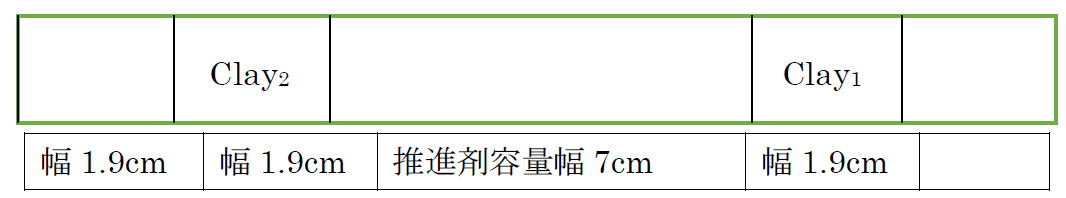
\includegraphics[height=1.5cm,clip]{okada/image/ki.png}
  \caption{木の棒}
  \label{fig:ki}
\end{figure}
この木の棒のメモリにしたがって塩ビパイプの中に推進剤を詰め込んでいく。Clayと書いた幅1.9cmの箇所には砂などを使用すれば良い。
 これに従って詰められたら次は燃焼用の穴をあける。ここでドリルビットを使用する。上に詰めているClay2に穴をあけないように注意する。
 以上でロケットエンジンの完成である。非常に簡単なものだ。[3]
\section{数種の推進剤の混合比表}
\subsection{硝酸カリウムと砂糖、アルミ粉末、硫黄}
推進剤の能力を引き上げる為にアルミやマグネシウムなどの金属粉末がよく使用される。
\begin{table}[H]
\caption{推進剤混合比表}
\centering
\begin{tabular}{c||c|c|c|c}
推進剤材料    &$P_1$ (\%)	&$P_2$ (\%)	&$P_3$ (\%)	&$P_4$ (\%)\\ \hline
硝酸カリウム  &60	         &60	       &60         &50\\
粉砂糖       &20          &10         &10         &10\\
アルミ粉末	  &15	          &20	&25	&25\\
硫黄	&5	&10	&5	&15\\ \hline
\end{tabular}
\end{table}

\subsection{硫黄と亜鉛粉末}
硝酸カリウムと砂糖などの混合推進剤に続いて愛好家の間で知られているのが硫黄と亜鉛粉末の混合による推進剤である。これらの混合による推進剤は大変力強い推進力が得られるが、適切な混合比および適切なノズルを付けなければ力が大きすぎたり、小さすぎたりする。制御が難しいためエンジン試験からは除外した。一般的に硫黄が34\%付近、亜鉛粉末が66\%付近で混合されるようである。
 亜鉛と硫黄の混合火薬については[付録B]に実験報告を記載している。


\begin{table}[H]
\caption{推進剤混合比表}
\centering
\begin{tabular}{c|c}
  推進剤材料	&P (\%)\\ \hline
  硫黄	&34近傍\\
  亜鉛粉末	&66近傍\\ \hline
\end{tabular}
\end{table}

\section{エンジンの保管}
さて出来上がったところでエンジンの保管はどうすれば良いのだろうと普通は考えるだろう。硝酸カリウムは吸湿性がないため保管は容易だ。ならば砂糖はどうだろうか。砂糖は水によく溶ける。つまり、砂糖は吸湿性が良いのである。
 吸湿性が良いということは空気中にさらしておけば当然べたべたになってくる。いくら乾燥材を使って湿気を取り除いたとしても反応を遅らせるだけである。
 実際にどれぐらいの期間保管できるかを観測した結果、乾燥材を入れた容器中で7日。空気中にさらした屋内で5日であった。したがって今回のエンジンでは長期間の保管は望めない。エンジンは使用する直前に用意するか、ほんの2、3日前に用意して乾燥材の中で保管するのがベストだろう。
 また当然であるが水分を含み、べたべたになったエンジンは使用できない。

\section{点火機構の制作}
点火機構はいくつか考えられる。一番経済的なのがサイリスタを用いて100円ショップなどで売っているキッチンタイマを利用するのが良い。その他にはIC555を使った簡単なタイマ回路などがある。
サイリスタを用いたタイマを考えよう。キッチンタイマのスピーカのプラス側をサイリスタのゲート側に繋ぐ。アノードには電源のプラス側がつながる。タイマをセットし、スピーカが鳴った時、サイリスタはオン状態となりダイオードと変わらない動作をする。つまり、アノードからカソードへ電流が流れるのである。ここでゲート信号を切断したとしても電流は流れ続ける。
サイリスタの等価回路を考えるとPNPトランジスタとNPNトランジスタを繋いだものを図示することが出来る。
\section{数種の推進剤の試験結果}
\subsection{試験結果}
次の3種類の推進剤を使い試験を行った。いずれも容器、ノズル、点火方法は同じである。
\begin{table}[H]
\caption{推進剤混合比表}
\centering
\begin{tabular}{c||c|c|c}
  推進剤材料	&$P_1$ (\%)	&$P_2$ (\%)	&$P_3$ (\%)\\ \hline
硝酸カリウム	&65	&60	&60\\
粉砂糖	&35	&20	&10\\
アルミ粉末	&―	&15	&20\\
硫黄	&―	&5	&10\\ \hline
\end{tabular}
\end{table}
以下に示す写真はそれぞれ$P_1, P_2, P_3$の実験写真である。
\begin{figure}[H]
  \centering
  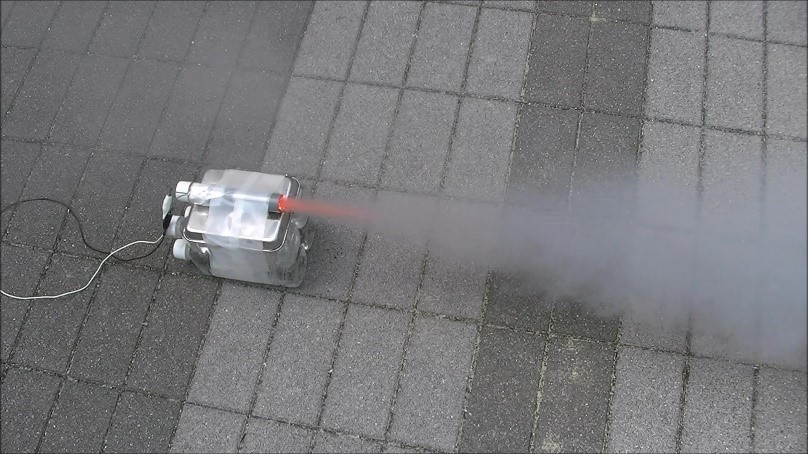
\includegraphics[height=3cm,clip]{okada/image/p_1.jpg}
  \caption{$P_1$試験}
  \label{fig:p1}
\end{figure}
\begin{figure}[H]
  \centering
  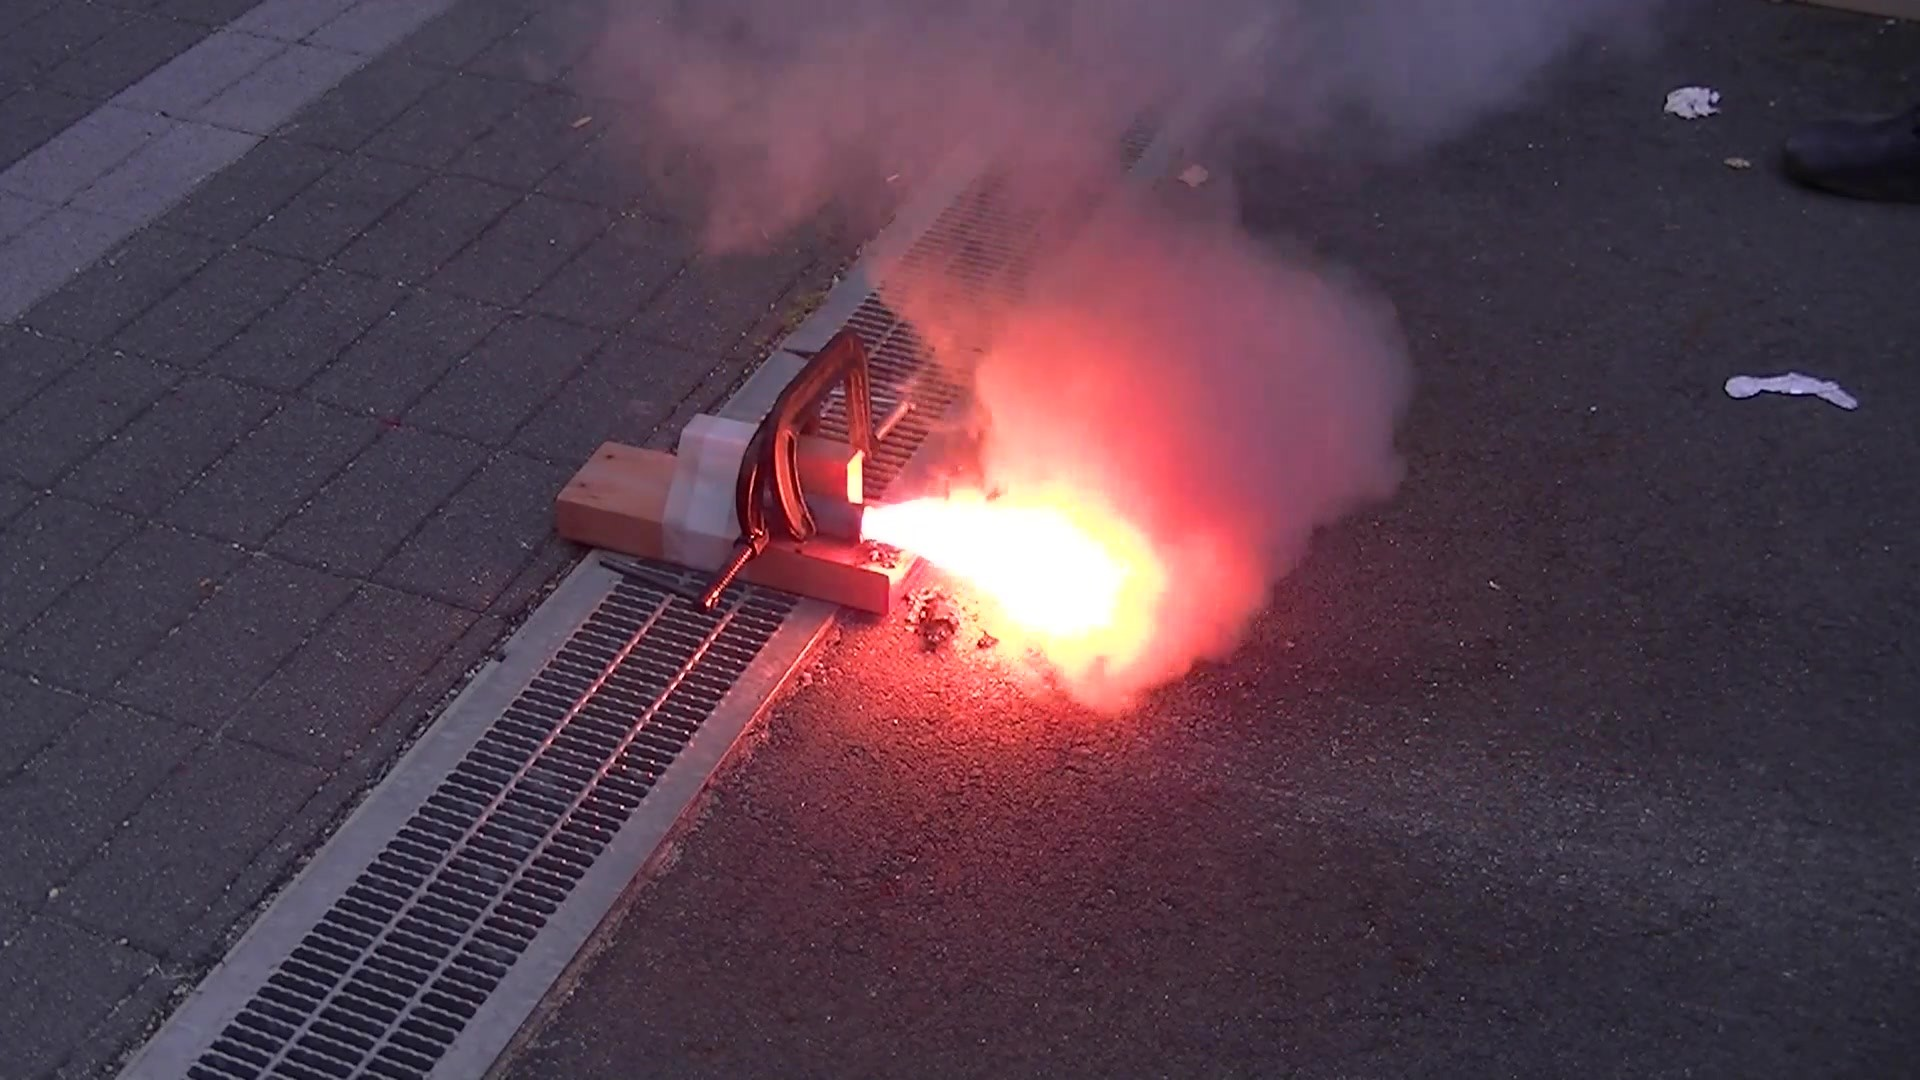
\includegraphics[height=3cm,clip]{okada/image/p_2.jpg}
  \caption{$P_2$試験}
  \label{fig:p2}
\end{figure}
\begin{figure}[H]
  \centering
  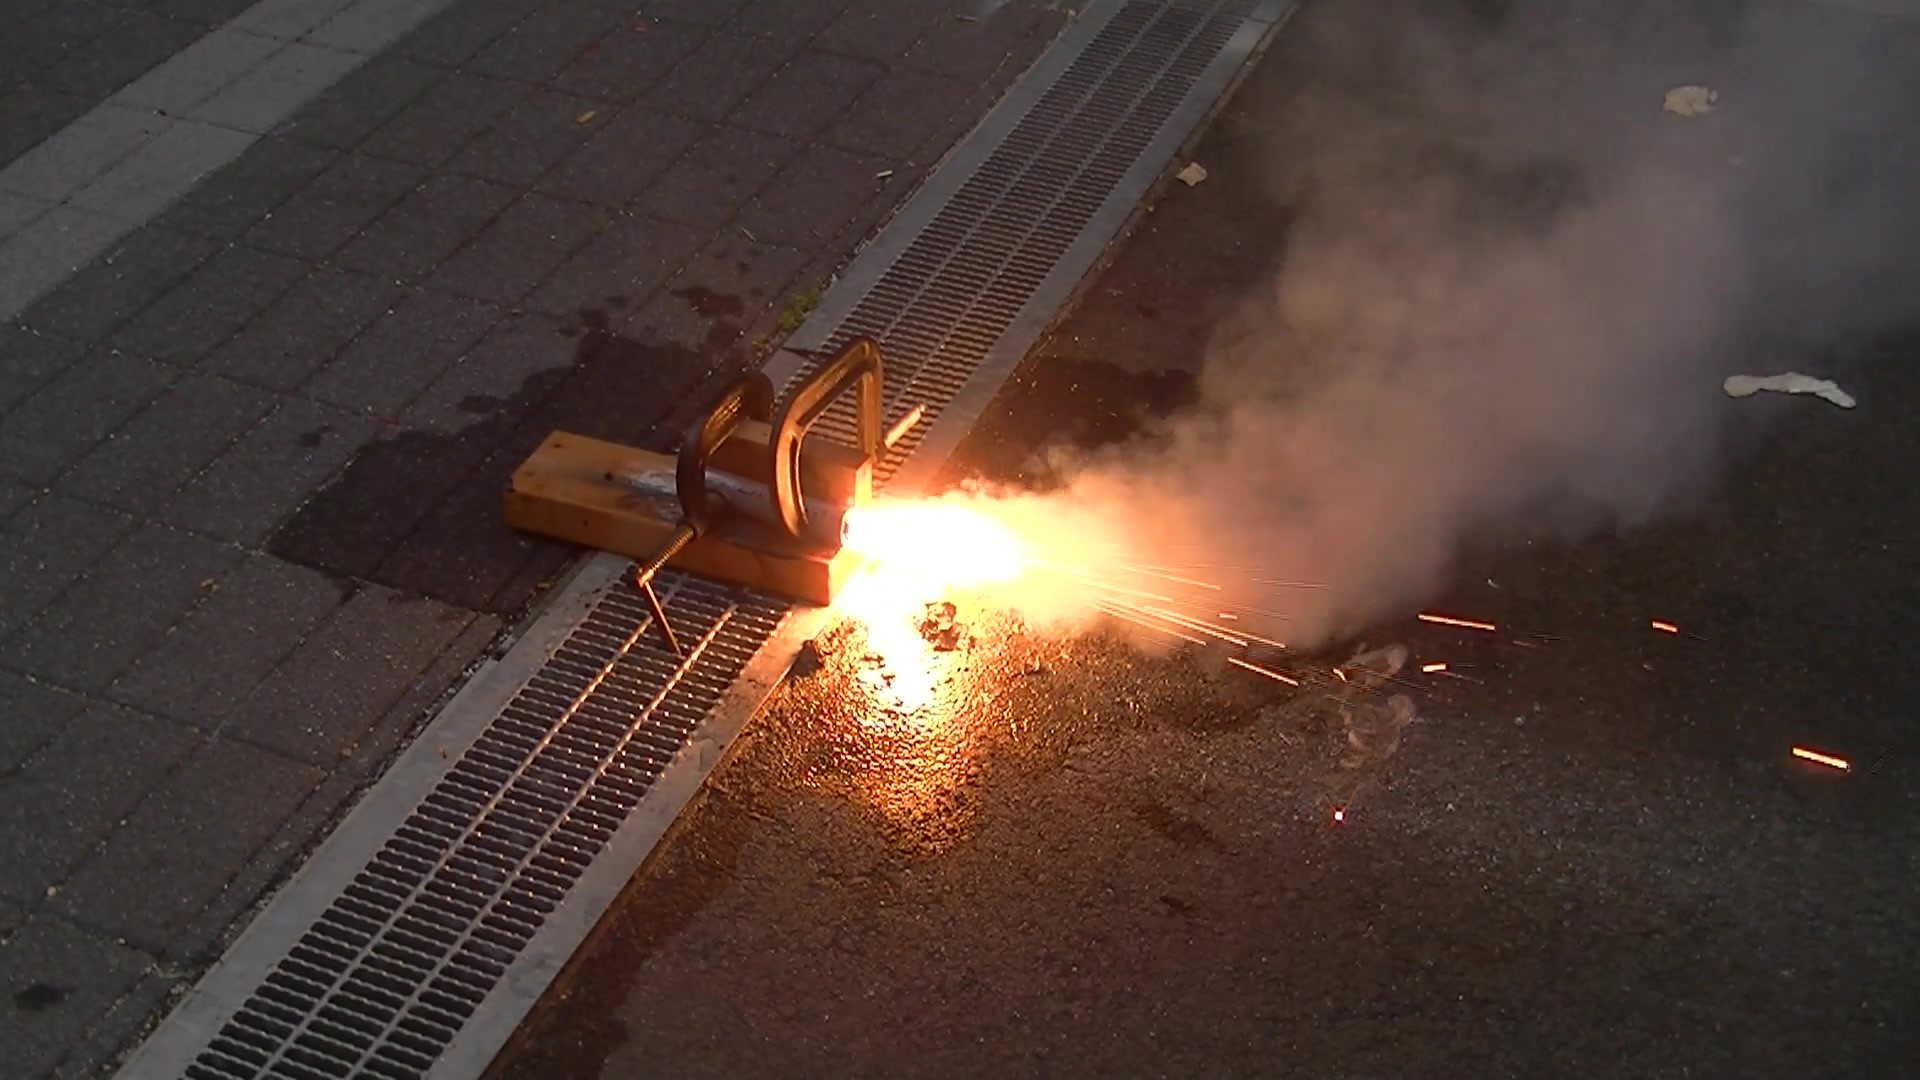
\includegraphics[height=3cm,clip]{okada/image/p_3.jpg}
  \caption{$P_3$試験}
  \label{fig:p3}
\end{figure}
$P_1$については問題なく安定して推進剤としての役割を果たしたが、$P_2$はただゆっくりと花火の様に燃焼しているだけであった。$P_3$は強力な推進剤となっていたが燃焼が不安定であった。
\subsection{試験結果の考察}
硝酸カリウムは酸素供給源であり、混ぜ合わせることで瞬間的に燃焼させることが出来る。噴射口は一つであるため、かかる圧力はすべて噴射口へと導かれ推進力が得られるとこういうことであろう。運動量保存則を考えれば良い。
 P2, P3の両試験において容器が溶けてしまったがこれはアルミ粉末を混ぜたことによって激しい反応を起こし、高温になったためと考えられる。対策として塩ビパイプよりも丈夫な容器を使えばよいだろう。

\section{ 【余談】 ロケット事件・大陸間弾道弾の実例と考察}
\subsection{中核派によるテロ事件から}
日本国内で無誘導弾の事件といえば革命的共産主義者同盟・中核派によるテロ事件が浮かび上がる。無誘導弾というよりは迫撃砲に近い。
 中核派のロケットは推進剤をロケットに詰め込んで発射させるのではなく黒色火薬を発射筒にセットして点火、発射させていたようである。
昔の火縄銃と同じで火薬を詰め込み、弾丸を込め、火をつけて発射するという大変古典的な方法を用いている。飛距離は2kmから4kmと結構な距離を記録しており、ただ単に火薬量が多かったからかロケットの形状がきっちりと計算されていたのかのどちらかが考えられる。複数の資料を見るにおそらく形状が良かったものと推測される。[4]
このころ(昭和50,60年代)なら普通、理科の実験などで塩素酸塩系をベースに推進剤が作られていたが塩素酸塩系は暴発しやすいため度々事故が起こっていた。[5]これを考えれば黒色火薬の燃焼による発射は比較的安全である。また慣性的エネルギーのみの飛行なので飛行中のエンジンの火薬質量を考慮せずに済み諸計算は大変楽である。
 発射後の話であるが、発射は上手くいっているにも関わらず信管の設計が難しかったようでほとんどが不発となっている。信管などの詳しいことは別の紙面にて述べる。

\subsection{朝鮮の弾道弾の発射試験から}
今日の朝鮮の弾道弾の発射試験の成果は目覚ましいものがある。1990年の弾道弾発射試験から今日までの実験を見ていればそれは明らかである。また2015年1月のSLBMの発射から2016年8月24日のSLBM発射試験でもそれは表れている。
2016年8月25日の朝鮮中央放送でSLBM発射についてアナウンサーが『主体朝鮮の核攻撃能力を一大誇示した。敬愛する金正恩同志の指導の下に戦略潜水艦弾道弾水中発射が正常に行われた』と述べており今まで以上にその発言が真実味を帯びているのを実感し、恐怖した。朝鮮の古い言葉に千里馬というのがあるが今は万里馬という時代語が使われ「千里馬よりも遥かに速く駆けていく」の意味がある。今が正にそれである。専門家が予想していたよりも我々が予想していたよりも朝鮮は速くに核弾頭を搭載する弾道弾の試験を行っている。また建国記念日である2016年9月9日には小型核弾頭の実験が敢行され核戦争の勢いである。一体朝鮮はどこに向かって速く駆けているのか。
さて今回行われた弾道弾の水中発射であるが、以前とはどこが違うのか。それは液体燃料と固体燃料の違いにある。液体燃料は注入したそばから揮発していくためすぐに打ち上げなければならない。その点、固体燃料であればある程度保管が出来るため使い勝手が良い。よって世界のトレンドは今や固体燃料である。
共和国朝鮮はソ連のコピー品のものを使っていたため液体燃料がトレンドであったが、方針を転換したのか固体燃料に切り替えたようだ。そこが前回とは違う点である。
次に掲載する写真は2016年8月25日に放送された朝鮮中央放送の一場面である。一段目左から「SLBM北極星本体写真」、「飛行1」、「飛行2」である。[6]

\begin{figure}[H]
  \centering
  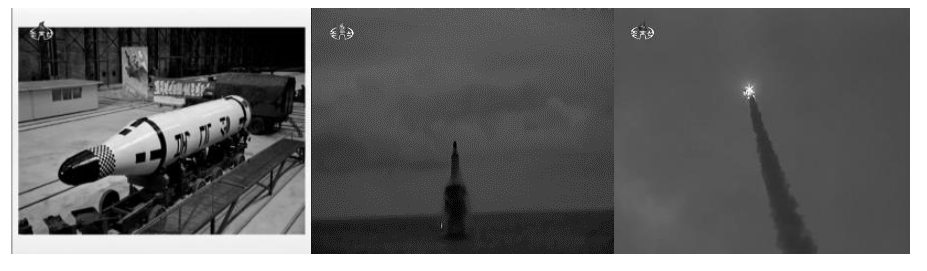
\includegraphics[height=3cm,clip]{okada/image/9no.png}
  \caption{本体写真、発射写真}
  \label{fig:9no}
\end{figure}

\newpage
\section*{参考文献}
\begin{enumerate}
  \item	火薬取締法及び航空法
  \item 佐々宏一著,「火薬工学」(森北出版, 2013年, p.3)
  \item JASON SMILEY, “EASY PVC ROCKETS”, 2005
  \item 複数セクトによる事件の被害及び犯行使用物の詳細資料(昭和60年~61年)
  \item 高等学校における火薬類の実験について(通産省, 昭和55年)
  \item \url{http://www.dprktoday.com/} (2016年8月25日配信の動画)
\end{enumerate}


\section{付録A 自家製ロケットエンジン高度計算手順}
ロケットの全重量:M(kg)\\

ロケットの直径:A($m^2$)=$\pi r^2$\\

空気抵抗力:$0.5\rm{Rho}\rm{Cd}\rm{A}v^2$\\
 Rho(空気の密度)=1.2($kg/m^3$)\\
 Cd(空気抵抗)=0.75(平均的な空気抵抗)\\
 まだ速度はわからないので速度を含めず計算する。これをkとする。\\

燃焼時間:$t=1/T$(sec)\\

重力加速度:$Mg=9.8M$\\

$q,x$の2つの値を次の様に定義する。\\
$q=\sqrt{[T-Mg]/k}$ Tは平均推力\\
$x=2kq/M$\\

完全燃焼速度:$v=q\frac{1-\exp{-xt}}{ 1+\exp{-xt}}$\\

動力飛行:$yb=\frac{-M}{2k}\ln \frac{T-Mg-kv^2} {T-M*g}$\\
慣性飛行:$yc=\frac{+M}{2k}\ln \frac{Mg+kv^2} {Mg}$\\

$yb+yc=Total\ Altitude$

\section{付録B 亜鉛と硫黄の混合火薬}
 粉末状の亜鉛と硫黄を混合し、点火すると激しく燃焼する。そのため高価な硝酸カリと粉糖による固体燃料の代替品、強化版として効果が期待できる。今回、亜鉛と硫黄の混合比率を変えてどのような挙動をするか観察することにした。
以下亜鉛をZ、硫黄をSと呼称する。
○条件○
次の3つに条件をわけて実験する。
\begin{itemize}
\item Z:50%、S:50%
\item Z:70%、S:30%
\item Z:80%、S:20%
\end{itemize}
\begin{figure}[H]
  \centering
  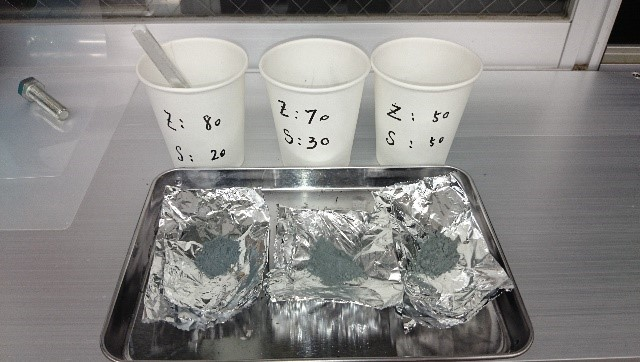
\includegraphics[height=4cm,clip]{okada/image/B.jpg}
  \caption{左からZ:80%, 70%, 50%}
  \label{fig:B}
\end{figure}
点火薬は黒色火薬(但、木炭の代りに粉糖を使用)1g程度を使用する。
\begin{itemize}
\item 手順
  \begin{itemize}
    \item 点火薬を使用せず点火、観察(各3g)
    \item 点火薬を使用して点火、観察(各3g)
    \item 3種を混合して点火、観察(各1g)
  \end{itemize}
\item 結果\\
この混合火薬は鈍感であり、点火薬がない場合ほとんど燃焼しない。亜鉛と硫黄のデータシートからわかるようにそれぞれ融解温度は500℃、400℃以上である。よってきっかけ(この場合は点火薬の黒色火薬)を与えてやればしっかりと燃焼する。
点火薬を使用した場合、Z,S50%はゆるやかに燃焼した。Z,S70%30%は燃焼が速かった(安定?)。Z,S80%20%はZ,S70%30%よりも燃焼速度が速く爆発的であった。これより、Zが増加するにつれ燃焼速度は増す傾向にあるのがわかる。
全てを混合した場合、まったく燃焼しなかった。混合比率はしっかりと計量する必要がある。
\end{itemize}
\begin{figure}[H]
  \centering
  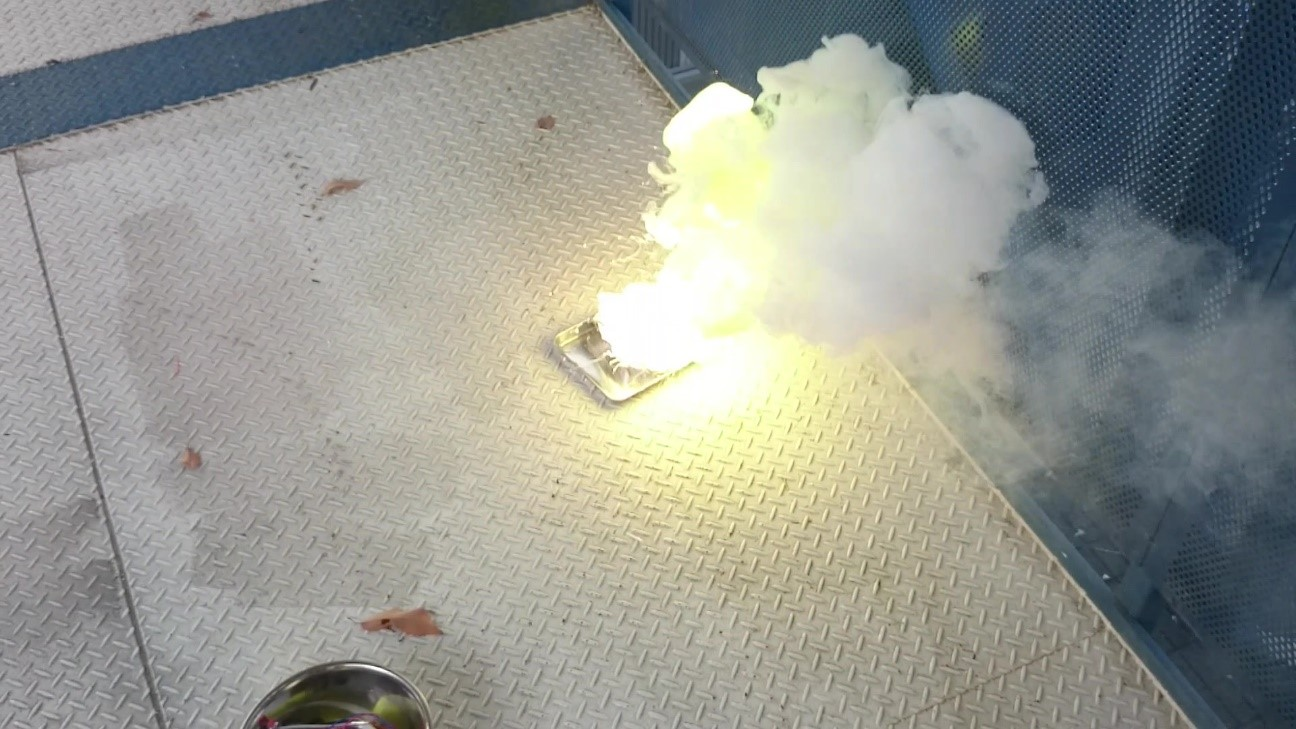
\includegraphics[height=4cm,clip]{okada/image/B_2.jpg}
  \caption{Z,S80%20%の燃焼}
  \label{fig:B}
\end{figure}

以上を踏まえると混合比率はZ > Sでなければ硝酸カリと粉糖の代替品にはならないことが理解できる。
亜鉛は500gで約1,500円と少々高いが硝酸カリウムは100gで約1,500円であるため固体燃料を制作するのであればコストの面から考えれば(制御面での難しさを除いて)、亜鉛と硫黄の混合火薬を使用するのが最善であろう。
 \clearpage


\backmatter %以降章番号を付けない。

\chapter*{物理科学研究会(旧核物理研)発足67周年に際して}
\addcontentsline{toc}{chapter}{物理科学研究会(旧核物理研)発足67周年に際して}
以前、同様の記事を書いたときに1959年発足としていたが、後輩と話し合った結果、又部室の大量の資料群から1949年の間違いであったことがわかった。本当かどうかも定かでないメモを無批判的に受け入れて記事に書き入れてしまったことは恥ずべきことである。今後はよくよく精査して記事を書かれたい。\par
立命館大学物理科学研究会は1949年に発足された研究会である。当時は物理科学研究会ではなく核物理研究会という呼称を使っていた。なぜ核物理研究会なのかというとこれは私の憶測であるが、その当時は「核」は夢のエネルギーとされており、研究も盛んであったということから核物理研究会となったのではないかと思われる。\par
1960年代ごろには超常現象班という班が創られた。UFOやヒエロニムスマシンなどの研究を行っていたようである。しばらくして消滅したが、1975年に復活して細々と活動を続けられていた。けれども、それも長くは続かず1990年頃に無くなってしまったと記録には書かれている。\par
そうして時代が変わり20世紀から21世紀に移行するとその時代にあった名称が必要なのではないかとの声があり、今の「物理科学研究会」となった次第である。\par
どうして名称変更されたのかは変更時(2000年)に発行された現役学生及びOBに向けた「変更にあたって」という文書に記載されていたがおおむね次に記述する様なことと同じであった。\par
研究会発足66周年を記念する2015年の8月1日にOB会があり、OB・現役生を含め15名が参加した。そこでOBの方に「核物理研究会に名前を戻したらどうだろうか」と提案を頂いた。\par
確かに名称も格好良いし、66年間の伝統を連綿と受け継いでいくという事は素晴らしいことであろう。\par
けれども、「核物理研究会」というのは我々の要求に即しているのだろうか。\par
「核物理」というのは原子・原子核・素粒子などの性質及び構造を研究する物理学である。そこで会員でない一般学生に立って考えてみると「核物理研究会」という名称は分野が一つだけなのかなと見られるわけである。つまり、\par
\begin{quote}
『核物理研究会は「核物理学」だけを研究しているのではなかったけれども、初めて見る人には「核物理学」だけの研究会に思えてしまう』
\end{quote}
とこういう訳なのだ。\par
「核」は物事・現象の中心という意味もあり、名称に加えたとしても不適当ではないとも考えられるのだが、やはり上記の事を考慮すれば「核物理」は不適当であると我々会員一同は統一した認識をしている。\par
「物理学」はこの世に存在するあらゆる自然現象を支配する法則を発見し、その帰するところを研究して体系化をはかり、理解に寄与する学問である。それ故、一般学生は「科学のあらゆることを研究することができるのだな」とこう考えることが出来る。\par
この点を踏まえて改めて見つめてみると、やはり今は「物理科学研究会」が適当であり、時代と学生の要求に即応していると言えるだろう。(「なぜ物理科学研究会か」岡田2016.01.06より)\par
上記の文書は新しく発行したものだがこれが21世紀に活動するにあたって名称を変更するに至ったおおよその経緯を説明しているものとする。\par
2010年以前はお隣のライフサイエンス研究会の様に子供たちのために科学教室を開いて教えていたこともあったと聞いたが、2010年あたりからはそのような活動はなくなりもっぱら自分たちの部屋でゼミを開き学祭で発表するだけの活動になったようである。\par
2014年は琵琶湖草津キャンパス(BKC)が京都から移転して「理工学部20周年」を迎え、さらに「電気電子工学科設立100周年」を迎えるという記念すべき年であった。それに伴って物理科学研究会も新しくホームページを開設したのである。\par
それから2015年に入ると3回生6人が退部し成員が減少してしまう痛手を負った。けれども成員減少をものともせずに日々自分自身の研究を進めている。\par
2015年の夏季休暇中には草津イオンモールからの依頼により子供たちの為に出張業務を行った。内容としては「子供に物理の楽しさを知ってもらうこと」とし、豆電球を使った電池の実験、ガウス加速器の実験、簡単電子オルゴール制作などを体験してもらった。\par
夏季休暇が終わった10月にも依頼を受け、ホバークラフト制作を体験してもらった。夏季休暇・10月の両体験とも子供たちには大変喜んでもらえたようで良かった。\par
お隣のライフサイエンス研究会は話を聞くところによれば「子供に科学の楽しさを教える」活動をしていると言う。我々は「物の理を科学、すなわち実験あるいは観察によって実証し、論理的に説明すること。そして、その自らが実証し説明した事柄をさらに深めて他人に伝える」活動をしている。そのため子供にわかりやすく教えるということが大変に難しくこれから視点を広げるにあたって、そこが我々にとっての問題点になるのは間違いない。\par
67周年を迎える今年、2016年にはお隣のライフサイエンス研究会幹部の方たちと話し合った結果、何か困ったこと技術力が欲しいことがあればお互いに協力し合うということを約束した。2016年が研究会にとって転機を向かえる年になるだろうことは想像に難くない。また会長の方針により今年から物理科学研究会は学祭を中心にした活動はやめ、ゼミ活動を中心に個人の研究活動・会誌の発行及び会外への配布などをすることとした。これから研究会はますます発展していくだろう。\par
物理科学研究会は時代の要求と理想を追求し続ける研究会である。大震災があってから「夢の核エネルギー」は潰えてしまった。けれども時代は新たなエネルギーの夢を追い求めることを要求している。\par
我々は長きに渡る研究会の探求精神を受け継ぎ、常に時代に即した目標を掲げて、時代の要求と理想とを追求し続けていかねばならない。\par
来年、物理科学研究会は発足68周年を迎える。もうすぐ70周年を迎える足音が近づいてきている。記念すべき研究会発足70周年を盛大に祝えるように後輩諸氏には努力を惜しまず前進前進と活動していってもらいたい。\par
\begin{flushright}
  \large 2016年8月31日\\
  \large 理工学部 電気電子工学科 岡田 優人
\end{flushright}



\end{document}
